\documentclass[a4paper]{article}

%Tutti gli usepackage vanno qui

\usepackage{geometry}
\usepackage[italian]{babel}
\usepackage[utf8]{inputenc}
\usepackage[T1]{fontenc}
\usepackage{tabularx}
\usepackage{longtable}
\usepackage{hyperref}
\usepackage{enumitem}
\hypersetup{
	colorlinks=true,
	linkcolor=black,
	filecolor=magenta,      
	urlcolor=blue,
}
% Numerazione figure 
\let\counterwithout\relax
\let\counterwithin\relax
\usepackage{chngcntr}

\counterwithin{table}{subsection}
\counterwithin{figure}{subsection}

\usepackage[bottom]{footmisc}
\usepackage{fancyhdr}
\usepackage{titlesec}
\setcounter{secnumdepth}{4}
\usepackage{amsmath, amssymb}
\usepackage{array}
\usepackage{graphicx}

%\usepackage{float}
\usepackage{layouts}
\usepackage{float}
\usepackage{eurosym}


\usepackage{layouts}
\usepackage{float}
\usepackage{eurosym}

%Comandi di impaginazione uguale per tutti i documenti
\pagestyle{fancy}
\lhead{
\includegraphics[scale=0.07]{res/images/logo8_crop.png}}
%Titolo del documento
\rhead{\doctitle{}}
\rfoot{\thepage}
\cfoot{}
\setlength{\headheight}{35pt}
\setcounter{tocdepth}{4}
\setcounter{secnumdepth}{4}
\renewcommand{\footrulewidth}{0.4pt}

% multirow per tabelle
\usepackage{multirow}

% Permette tabelle su più pagine

%\usepackage{longtable}


% colore di sfondo per le celle
\usepackage[table]{xcolor}

%COMANDI TABELLE
\newcommand{\rowcolorhead}{\rowcolor[HTML]{56A5EC}} %intestazione 
\newcommand{\rowcolorlight}{\rowcolor[HTML]{fafafa}} %righe chiare/dispari
\newcommand{\rowcolordark}{\rowcolor[HTML]{e1f5fe}} %righe scure/pari
\newcommand{\colorhead}{\color[HTML]{FFFFFF}} %testo intestazione
\newcommand{\colorbody}{\color[HTML]{000000}} %testo righe
\newcommand{\tabitem}{~~\rlap{\textbullet}~~}

\newcommand{\glo}{$_{G}$}
\newcommand{\glosp}{$_{G}$ }

\definecolor{pari}{HTML}{E1F5
\definecolor{dispari}{HTML}{FAFAFA}


%Lista dei comandi personalizzati
\newcommand{\doctitle}{Verbale interno 2019-02-20}
\newcommand{\rev}{1.0.0}
\newcommand{\approv}{}
\newcommand{\ver}{}
\newcommand{\red}{Matteo Santinon}
\newcommand{\stato}{Approvato}
\newcommand{\uso}{Interno}
\newcommand{\describedoc}{Riassunto dell'incontro del gruppo \textit{8Lab 
Solutions} tenutosi il 2019-02-20.}
\newcommand{\destinatari}{8Lab Solutions\\& Prof. Tullio Vardanega\\& Prof. Riccardo Cardin}




\makeindex

\begin{document}

\thispagestyle{empty}
\begin{titlepage}
	\begin{center}
		
\includegraphics[scale = 0.3]{res/images/logo8_crop.png}\\
		\large \textbf{8Lab Solutions - Progetto "Soldino"} \\
		\vfill
		\Huge \textbf{\doctitle}
		\vspace*{\fill}
        
        \vfill
        \large
        \begin{tabular}{r|l}
                        \textbf{Versione} & \rev{} \\
                        \textbf{Approvazione} & \approv{} \\
                        \textbf{Redazione} & \red{} \\
                        \textbf{Verifica} & \ver{} \\
                        \textbf{Stato} & \stato{} \\
                        \textbf{Uso} & \uso{} \\
                        \textbf{Destinato a} & \parbox[t]{5cm}{8Lab Solutions
                        \\Prof. Tullio Vardanega\\Prof. Riccardo Cardin}
                \end{tabular}
                \vfill
                \normalsize
                \textbf{Descrizione}\\
                \describedoc
                \vfill
                \small
                \texttt{8labsolutions@gmail.com}
	\end{center}
\end{titlepage}


\pagebreak
\section*{Tabelle delle modifiche}
\renewcommand{\arraystretch}{1.5}
\begin{center}
\begin{longtable}{ >{\centering}p{1.5cm} >{\centering}p{1.8cm}
                   >{\centering}p{2.9cm} >{\centering}p{2cm} >{}p{5cm} }

\hline
\textbf{Versione} & \textbf{Data} & \textbf{Nominativo} & \textbf{Ruolo} &
\textbf{Descrizione} \tabularnewline \hline
				1.0.0 & 2018-12-26 & Francesco Donè & \textit{Responsabile} & Approvazione 
				del documento.
				\tabularnewline
				\hline
				0.1.0 & 2018-12-23 & Matteo Santinon & \textit{Verificatore} & Modifica e revisione del documento.
				\tabularnewline
				\hline
				0.0.2 & 2018-12-22 & Giacomo Greggio & 
				\textit{Analista} & Stesura documento.
				\tabularnewline
                \hline
                0.0.1 & 2018-11-25 & Mattia Bolzonella & 
                \textit{Analista} &
                Creata struttura del documento in \LaTeX{}.
                \tabularnewline
               \hline
                       
        %\end{tabularx}
        \\
        
\end{longtable}
\end{center}
\renewcommand{\arraystretch}{1}

\counterwithin{table}{subsection}
\counterwithin{figure}{subsection}

\pagebreak

\tableofcontents

\pagebreak

\listoffigures

\pagebreak

\listoftables

\pagebreak

\counterwithin{table}{subsection}
\counterwithin{figure}{subsection}
\section{Informazioni generali}

\subsection{Informazioni incontro}
\begin{itemize}
\item \textbf{Luogo}: Dipartimento di Matematica "Tullio Levi-Civita";
\item \textbf{Data}: 2019-03-18;
\item \textbf{Ora di inizio}: 10:15;
\item \textbf{Ora di fine}: 11:05;
\item \textbf{Segretario}: Matteo Santinon;
\item \textbf{Partecipanti}: 
\begin{itemize}
	\item Federico Bicciato;
	\item Mattia Bolzonella;
	\item Francesco Donè;
	\item Sara Feltrin;
	\item Giacomo Greggio;
	\item Samuele Giuliano Piazzetta;
	\item Paolo Pozzan;
	\item Matteo Santinon.
\end{itemize}
\end{itemize}

\subsection{Argomenti affrontati}
Nell'incontro si è parlato principalmente dell'esito della Revisione di 
Progettazione tenutasi il giorno 2019-03-15.


\pagebreak
\section{Analisi dei rischi}

\pagebreak
\section{Modello di sviluppo}
La scelta di un modello di sviluppo è fondamentale per la pianificazione di 
progetto e a tal fine è stato adottato il \textbf{modello incrementale}.

\subsection{Modello incrementale}
Il modello di sviluppo incrementale permette di suddividere lo sviluppo del sistema per 
incrementi, ognuno dei quali incorpora una funzionalità. \\
L'aggiunta, modifica e cancellazione di requisiti sono consentite previa discussione con il proponente e sua 
approvazione; tuttavia non sono permesse durante la fase di sviluppo dell'incremento corrente.\\
Questo modello di sviluppo si combina bene con il versionamento del sistema, che traccia le modifiche rendendole più visibili.\\
L'adozione di questo modello comporta i seguenti vantaggi:
\begin{itemize}
	\item le funzionalità primarie hanno priorità nello sviluppo, così che il proponente possa subito valutarle;
	\item si può ricevere il feedback del cliente frequentemente, anche ad ogni incremento;
	\item sviluppare per incrementi successivi limita gli errori al singolo incremento;
	\item le modifiche, l'individuazione e la correzione degli errori sono più economiche;
	\item anche le fasi di verifica e test sono facilitate, perché più mirate.
\end{itemize}
\subsubsection{Incrementi individuati} Durante i periodi di Progettazione Architetturale e Progettazione di Dettaglio sono stati individuati alcuni incrementi. Di seguito è riportato il tracciamento incremento-requisiti, in maniera tale da comprendere meglio quali requisiti vengono soddisfatti in ciascun incremento. \\ \\
I requisiti riportati nella tabella includono tutti i requisiti figli. Tutti i requisiti non riportati nella tabella sono da intendersi soddisfatti, in parte, da ogni incremento. 

%tabella tracciamento incremento-requisiti


\rowcolors{2}{pari}{dispari}

\begin{longtable}{ >{\centering}p{0.5\textwidth}
		>{\centering}p{0.5\textwidth}}
	\caption{Tabella di tracciamento incremento-requisiti}\\
	\rowcolorhead 
	\textbf{\color{white}Incremento}
	& \textbf{\color{white}Requisiti} 
	\tabularnewline 	
	\endfirsthead
	\rowcolor{white}\caption[]{(continua)} \\
	\rowcolorhead 
	\textbf{\color{white}Fonte}
	& \textbf{\color{white}Requisiti} 
	\tabularnewline 
	\endhead

	Incremento 1 - Registrazione	&	R2F1 \\
	R1F2	\tabularnewline
	Incremento 2 - Login	&	R1F3 \\
	R1F4	\tabularnewline
	Incremento 3 - Home	&	R1F8 \\
	R1F9 \\
	R1F10 \\
	R1F11 \\
	R1F12 \\
	R2F13 \\
	R1F14 \\
	R1F18 	\tabularnewline
	Incremento 4 - Pagina Governativa	&	R1F5 \\
	R1F6 \\
	R1F7	\tabularnewline
	Incremento 5 - Pagina Azienda	&	R1F15 \\
	R1F16 \\
	R3F17 \\
	R1F19	\tabularnewline
	Incremento 6 - Pagina Cittadino	&	R1F15	\tabularnewline
	
\end{longtable}



\pagebreak
\section{Pianificazione}
Alla luce delle scadenze presentate nella \hyperlink{scadenze}{sottosezione 2.5}, la pianificazione di progetto viene suddivisa nelle seguenti fasi:
\begin{enumerate}
	\item \textbf{Analisi};
	\item \textbf{Consolidamento dei requisiti};
	\item \textbf{Progettazione architetturale};
	\item \textbf{Progettazione di dettaglio e codifica};
	\item \textbf{Validazione e collaudo}.
\end{enumerate}
Ogni fase viene suddivisa in attività\glosp che verranno realizzate durante il 
periodo stabilito per la fase stessa. 
\subsection{Analisi}
\textit{Periodo: dal 2018-11-16 al 2019-01-14}\\
L'inizio del periodo di questa fase coincide con la data di formazione dei 
gruppo e la fine coincide con la data di consegna dei documenti relativi alla 
revisione dei requisiti. Questa fase è stata scomposta nelle seguenti sotto attività:
\begin{itemize}
	\item \textbf{Individuazione degli strumenti}: questa attività consiste nel 
	determinare quali strumenti il gruppo deve utilizzare per la comunicazione, per 
la stesura dei documenti e per il versionamento, lo sviluppo e la verifica del 
software; 
	\item \textbf{Norme di Progetto}: sono definite tutte le regole utili per lo svolgimento del progetto, relative al prodotto da realizzare e ai processi da adottare. Il documento \textit{Norme di Progetto} viene redatto dal Responsabile di progetto e dall'Amministratore;
	\item \textbf{Studio di fattibilità}: in questa attività gli Analisti effettuano uno studio sommario dei capitolati in modo da determinare quale di essi verrà scelto. Questa attività e da considerarsi bloccante per l'attività di \textit{Analisi dei Requisiti};
	\item \textbf{Analisi dei Requisiti}: durante questa attività vengono 
	identificati ed analizzati i requisiti del capitolato scelto nell'attività 
	di \textit{Studio di fattibilità} e il relativo documento viene composto dagli Analisti;
	\item \textbf{Piano di Progetto}: il Responsabile pianifica il 
	lavoro del gruppo 8Lab Solutions, inteso come suddivisione di compiti, 
	risorse e attività. Inoltre viene calcolato il preventivo per la realizzazione 
	del progetto. Questa attività comporta anche la stesura 
	del documento \textit{Piano di Progetto};
	\item \textbf{Piano di Qualifica}: in questà attività si individuano le 
	metodologie attraverso le quali si garatisce la qualità del prodotto. A supporto di ciò viene redatto il documento \textit{Piano di Qualifica} da parte degli Analisti; 
	\item \textbf{Glossario}: vengono individuati tutti i termini che possono risultare ambigui e 
	vengono definiti nel documento \textit{Glossario} che viene 
	redatto durante tutta la fase di analisi dei requisiti.
\end{itemize}

\begin{figure}[H]
	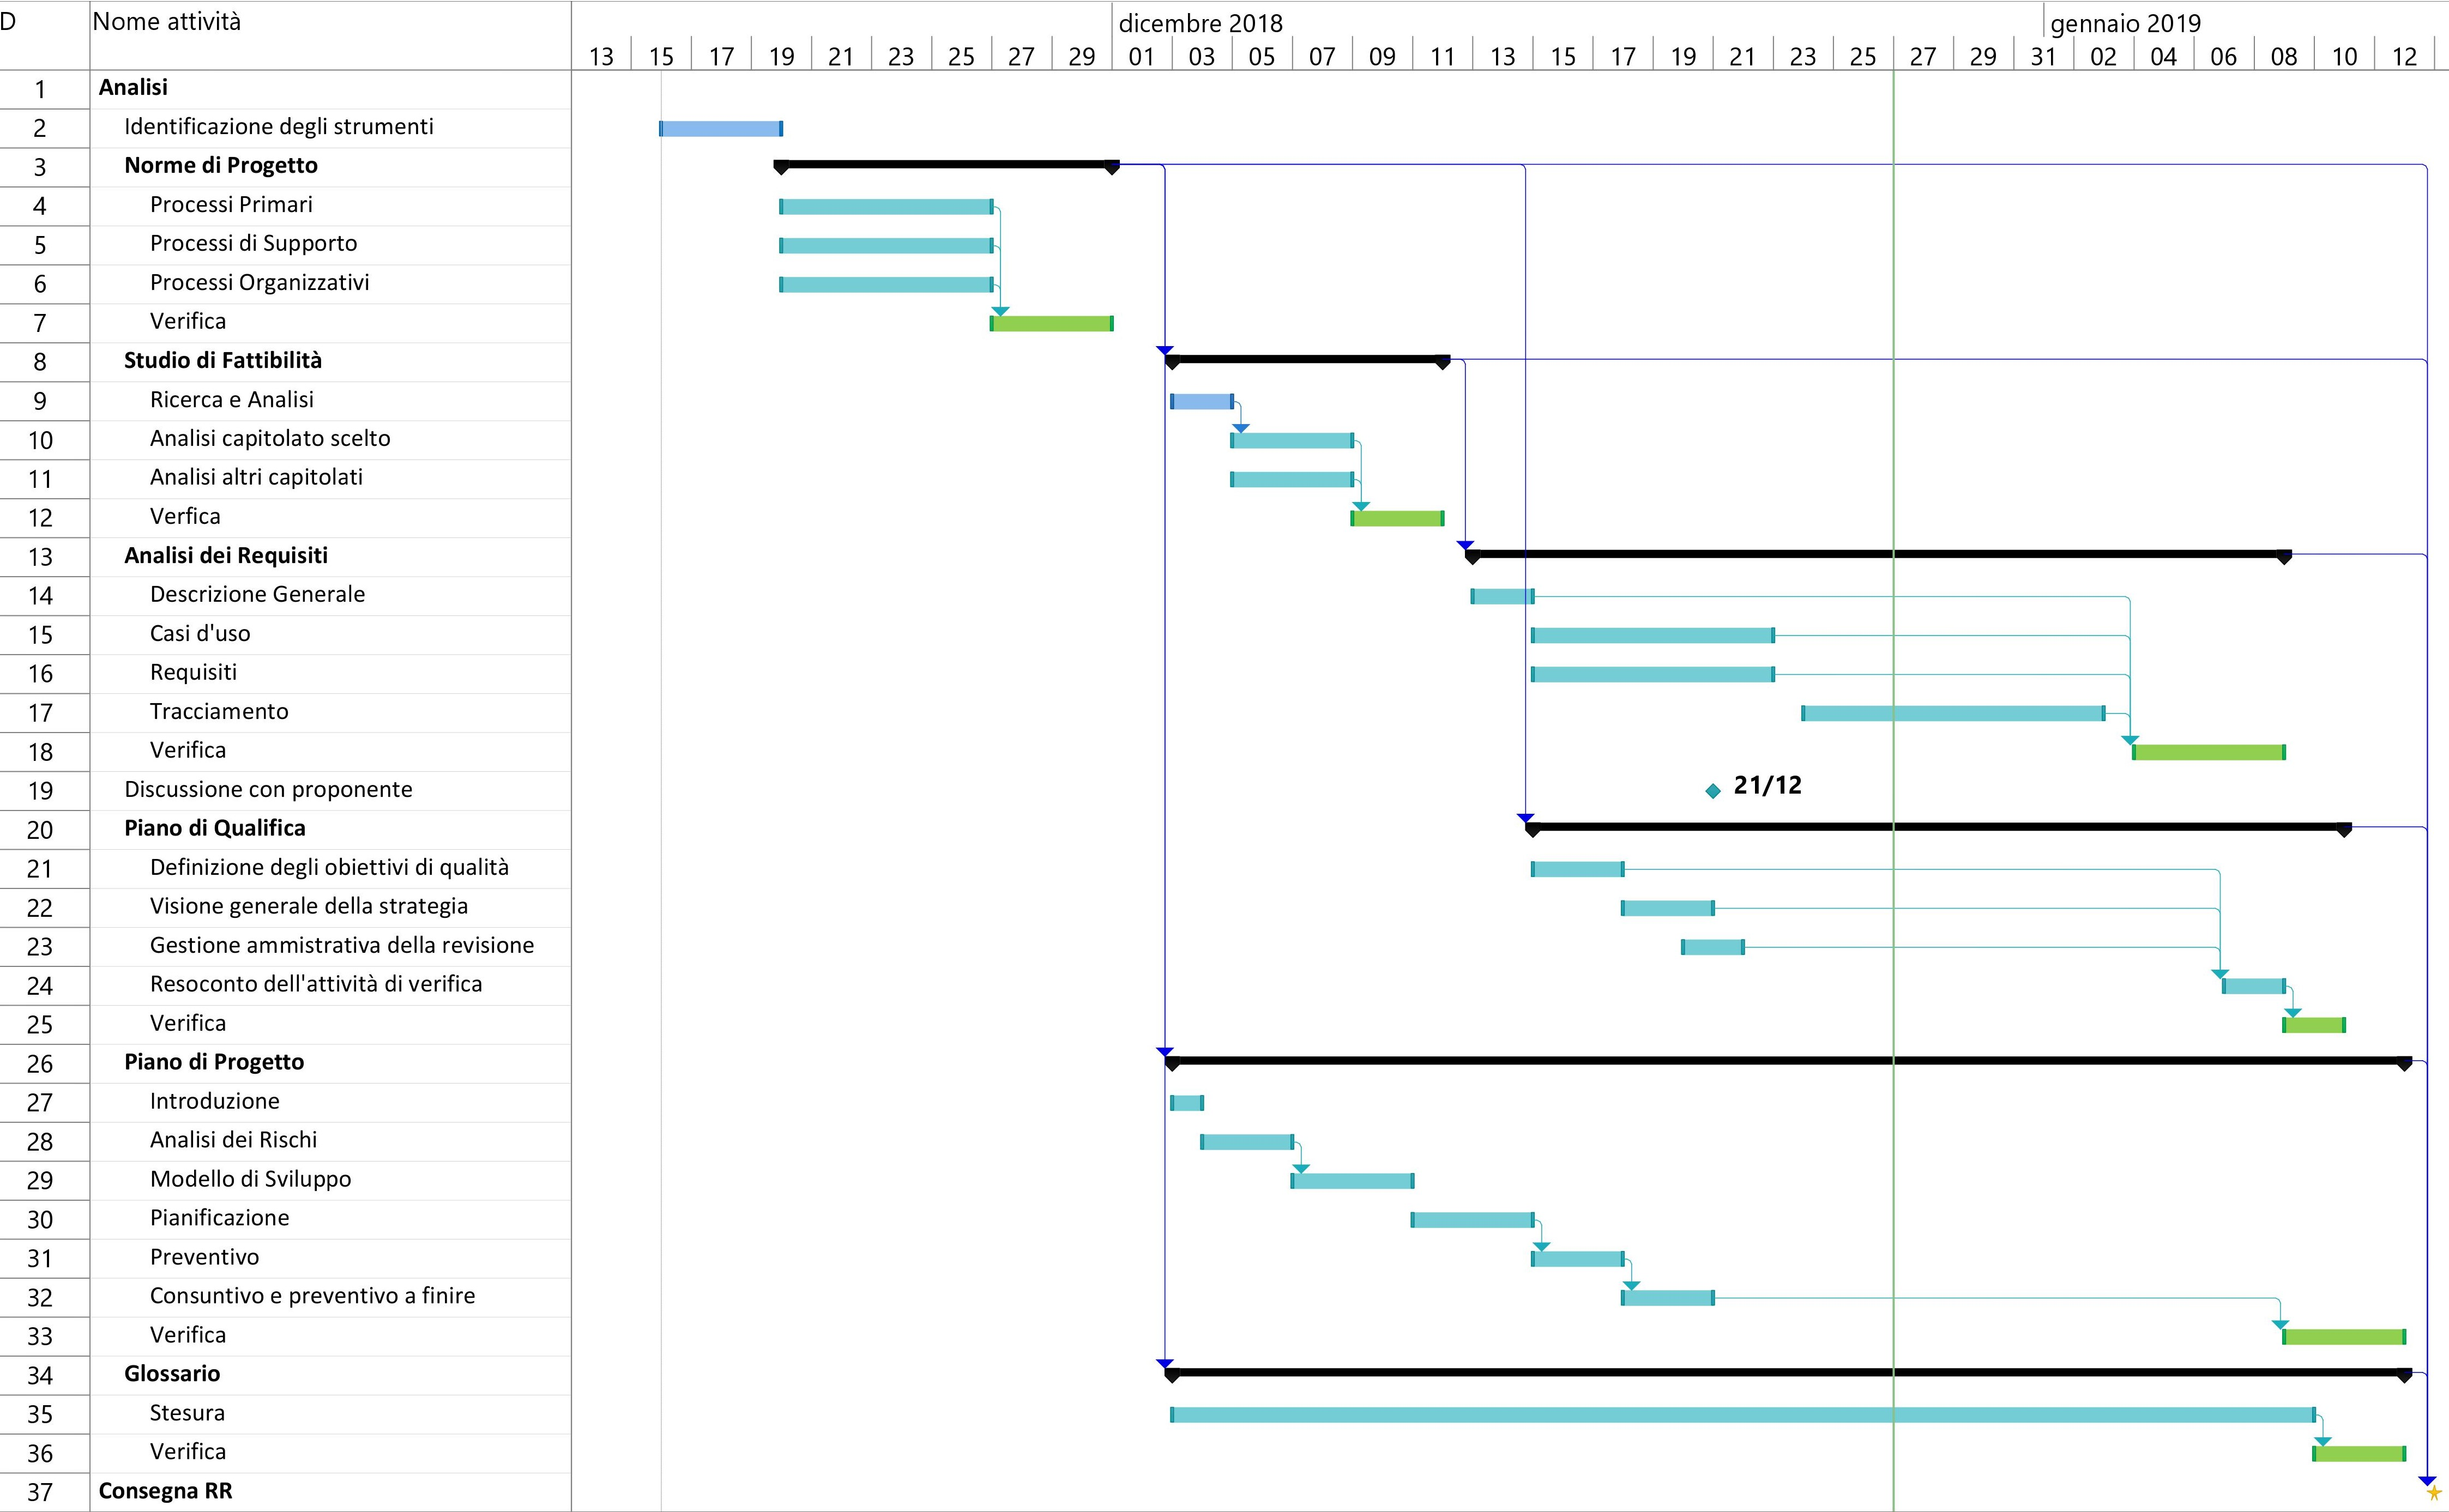
\includegraphics[width=0.99\linewidth]{res/images/gantt_analisi1.jpg}
	\caption{Diagramma di Gantt della fase di Analisi}
\end{figure}



\subsection{Consolidamento dei requisiti}
\textit{Perdiodo: dal 2019-01-14 al 2019-01-21} \\
Questa fase comincia con la fine della fase di \textit{Analisi} e termina il giorno della presentazione della \textit{Revisione dei Requisiti}. Le attività di questa fase sono:
\begin{itemize}
	\item \textbf{Consolidamento}: questa attività ha lo scopo di consolidare e migliorare i requisiti ottenuti nella fase precendente;
	\item \textbf{Incremento e Verifica}: se necessario vengono migliorati i documenti prodotti nella fase precendente.
\end{itemize}
Inoltre durante questa fase ogni componente del gruppo dovrà dedicare almeno 15 
ore di studio e approfondimento delle tecnologie necessarie alle prossime fasi 
e alla realizzazione del prodotto. Questa attività verrà gestita in modo 
autonomo dai membri del gruppo, quindi non sarà riportata nel diagramma di 
Gantt \ref{fig:gantt_con} sottostante.

\begin{figure}[H]
	\label{fig:gantt_con}
	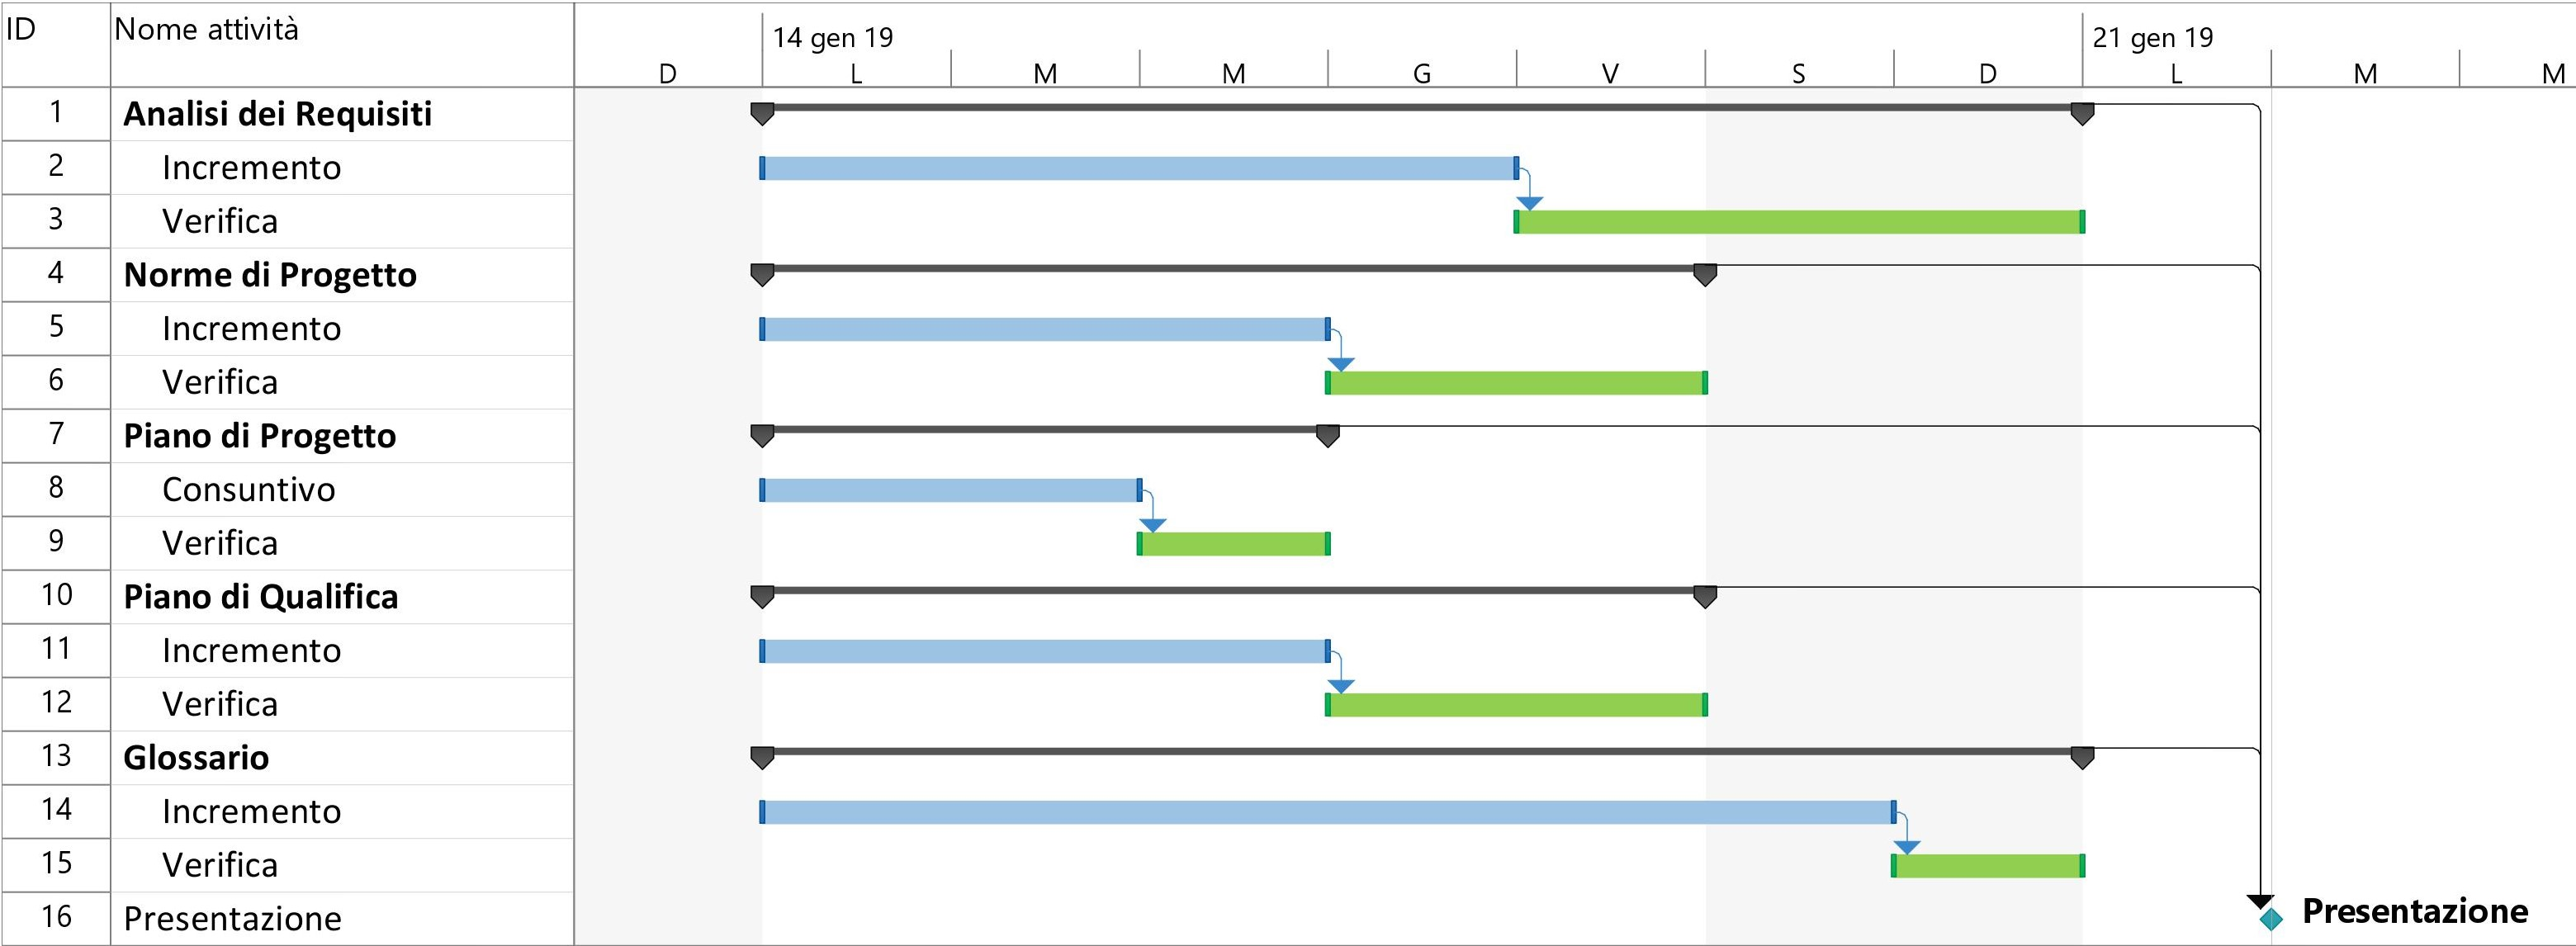
\includegraphics[width=0.99\linewidth]{res/images/gantt_cons.jpg}
	\caption{Diagramma di Gantt della fase di Consolidamento dei requisiti}
\end{figure}

%-----------------Sottosezione Progettazione Architetturale---------------------
\subsection{Progettazione architetturale}
\textit{Periodo: dal 2019-01-21 al 2019-03-08} \\
Questa fase comincia il giorno dopo la presentazione e la fine coincide con la data di consegna \textit{Revisione di 
Progettazione}. In questo periodo verrà individuata una soluzione architetturale 
tale per cui i requisiti richiesti vengano soddisfatti.
\begin{itemize}
	\item \textbf{Specifica Tecnica}: viene redatto il documento 
	\textit{Specifica Tecnica} nel quale vengono individuati i design 
	pattern\glosp che verranno adottati per lo sviluppo. Inoltre il documento 
	include il tracciamento dei requisiti.\\
	Infine viene codificato il \textbf{\textit{Proof of Concept}}\glosp il 
	quale viene presentato o condiviso tramite repository al committente e 
	proponente in una data da definirsi.
	\item \textbf{Incremento e Verifica}: se necessario vengono migliorati i 
	documenti prodotti nelle fasi precedenti.
\end{itemize}

\begin{figure}[H]
	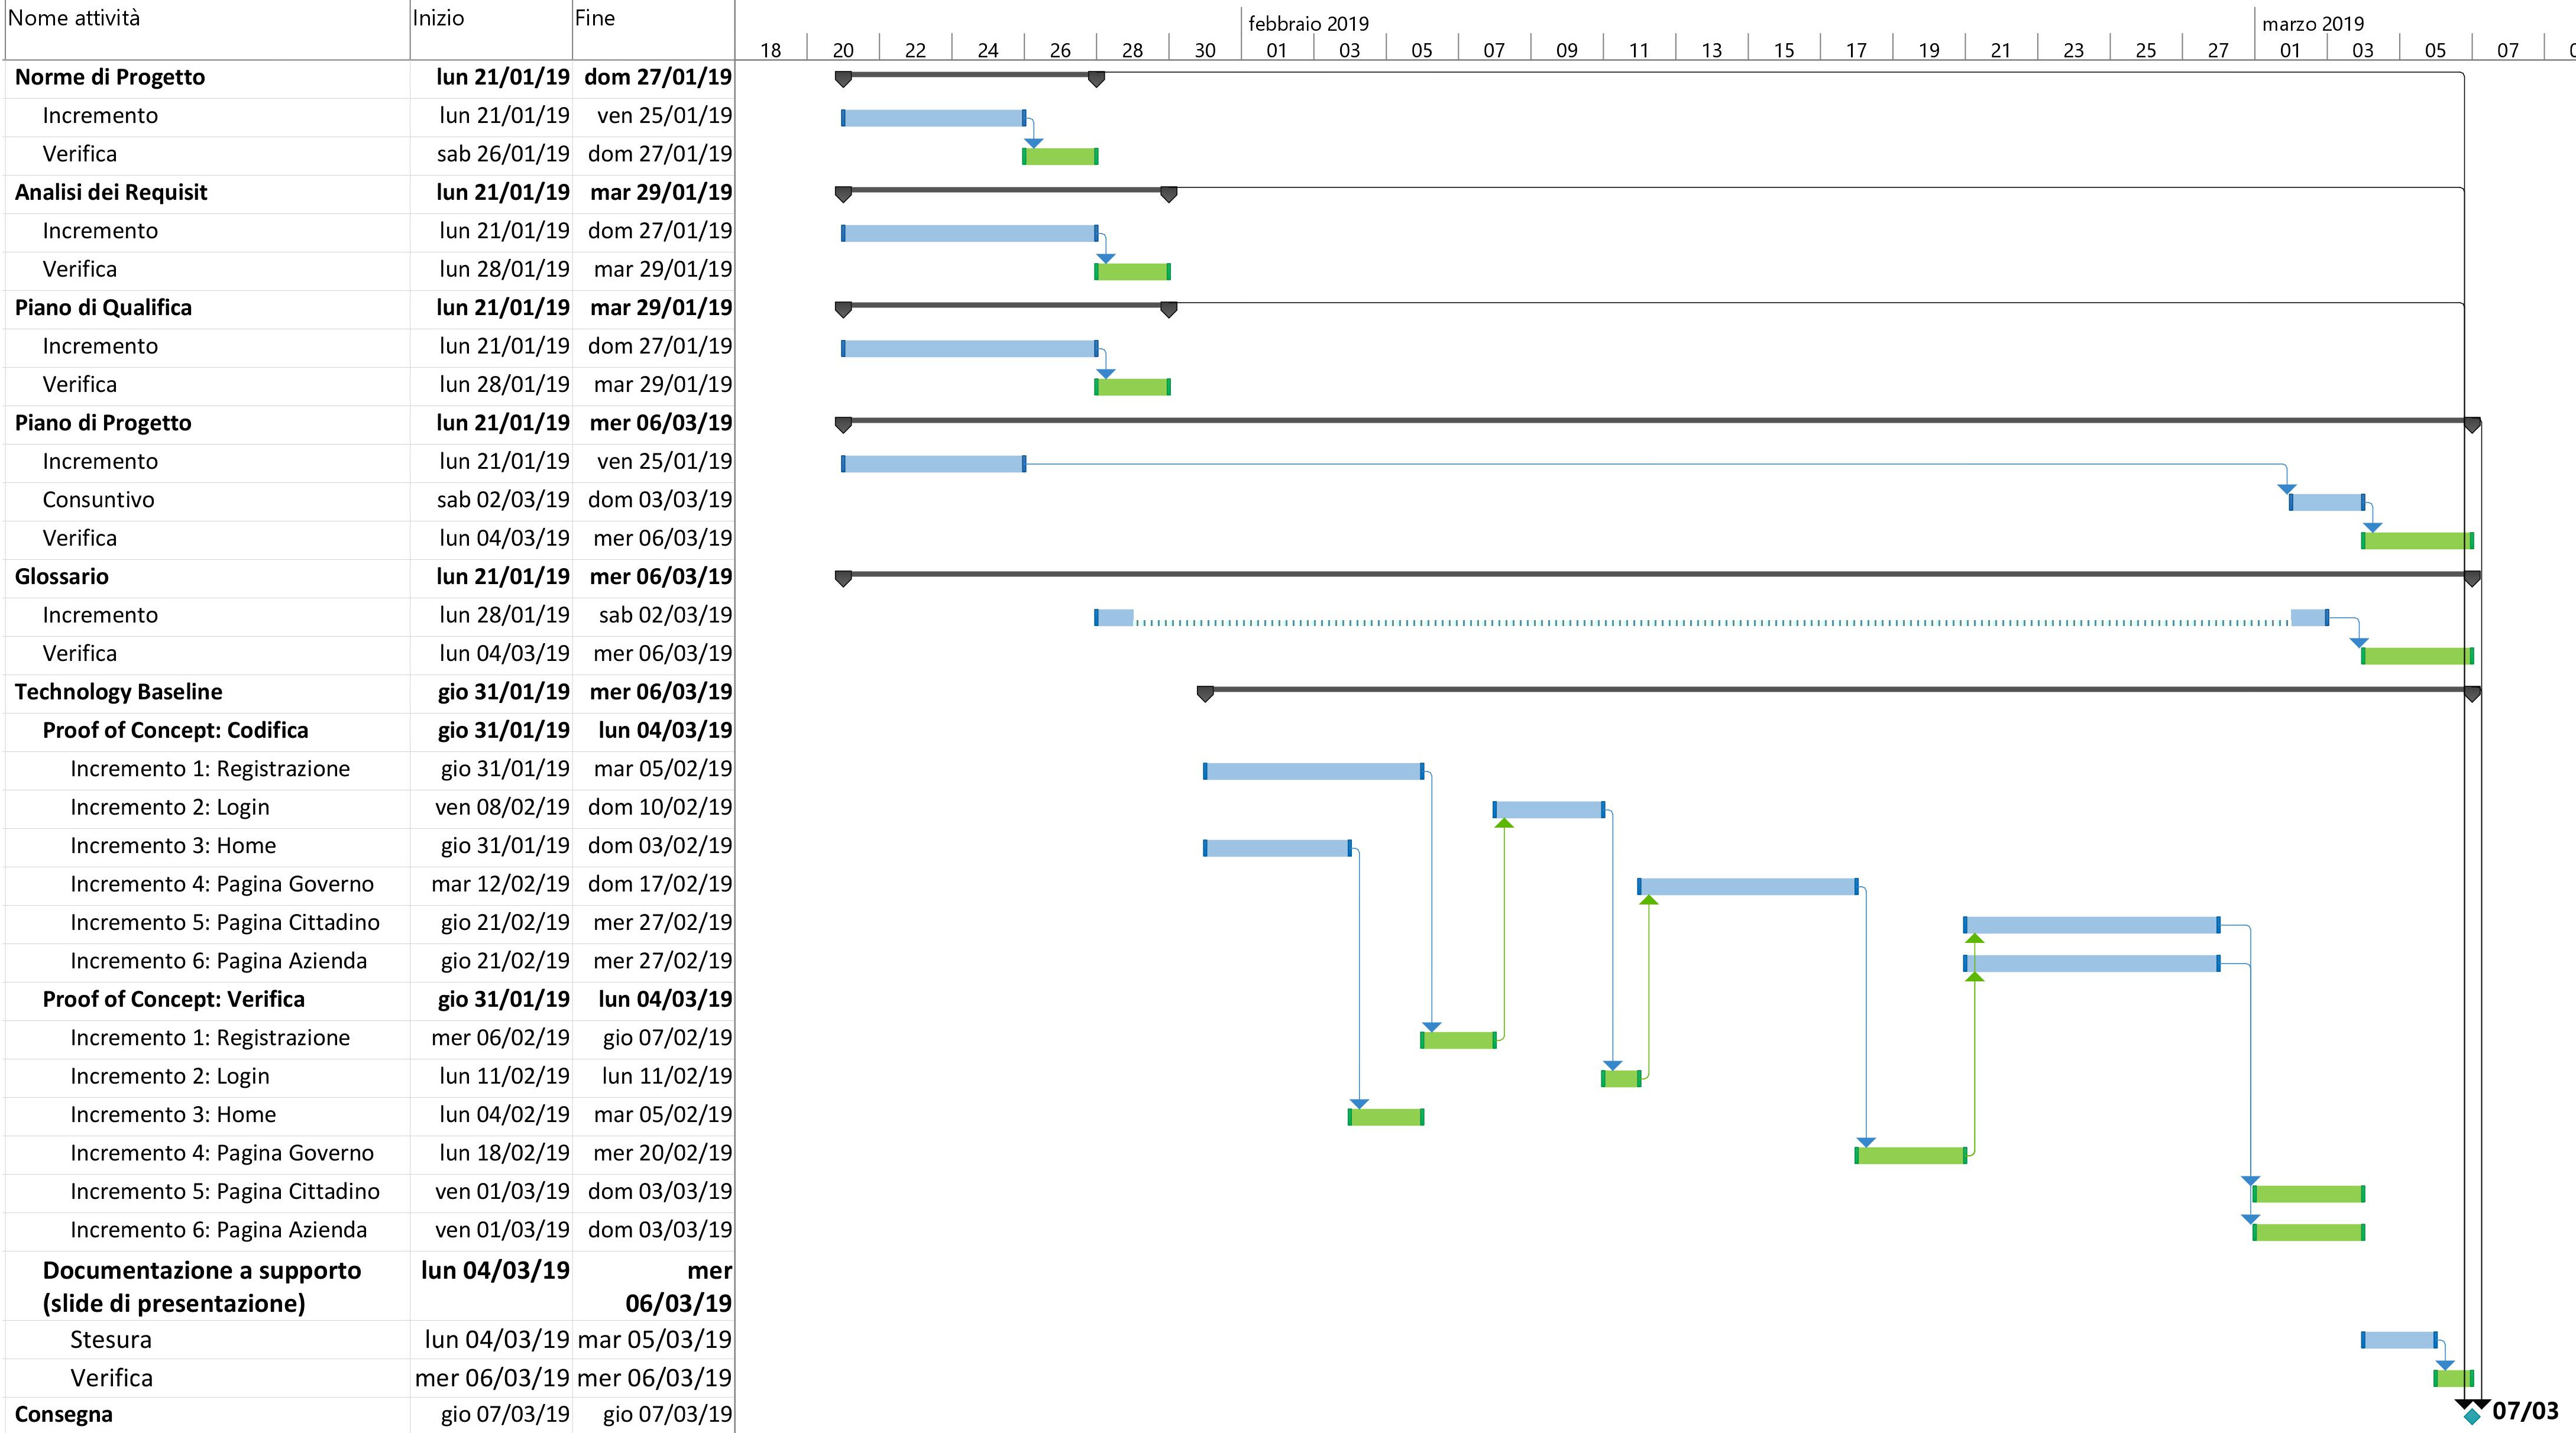
\includegraphics[width=0.99\linewidth]{res/images/gantt_pa.jpg}
	\caption{Diagramma di Gantt della fase di Progettazione architetturale}
\end{figure}


%-------------------Sottosezione Progettazione di Dettaglio---------------------
\subsection{Progettazione di dettaglio e codifica}
\textit{Periodo: dal 2019-03-15 al 2019-04-12}
L'inizio di questa fase è il giorno della scadenza della \textit{Revisione di 
Progettazione} e la data di fine coincide con la data di consegna dei documenti 
in vista della \textit{Revisione di Qualifica}. Le attività di questa fase sono:
\begin{itemize}
	\item \textbf{Definizione di Prodotto}: a seguito della \textit{Specifica 
	Tecnica} l'architettura individuata in essa viene scomposta nei suoi 
	componenti per esseri analizzati nel dettaglio in modo tale da fornire i 
	dettagli necessari alla codifica e alla verifica dei componenti. A supporto 
	di ciò viede redatto il documento \textit{Definizione di Prodotto};
	\item \textbf{Codifica}: questa attività consiste nella scrittura del 
	codice e della sua verifica con modalità e strumenti definiti nel 
	\textit{Piano di Qualifica v2.0.0}
	\item \textbf{Manuale Utente}: viene redatto il documento \textit{Manuale 
	Utente} atto a fornire istruzioni e indicazioni per l'utilizzo del prodotto;
	\item \textbf{Incremento e Verifica}: se necessario vengono migliorati i 
	documenti prodotti nelle fasi precedenti.
\end{itemize}


\begin{figure}[H]
	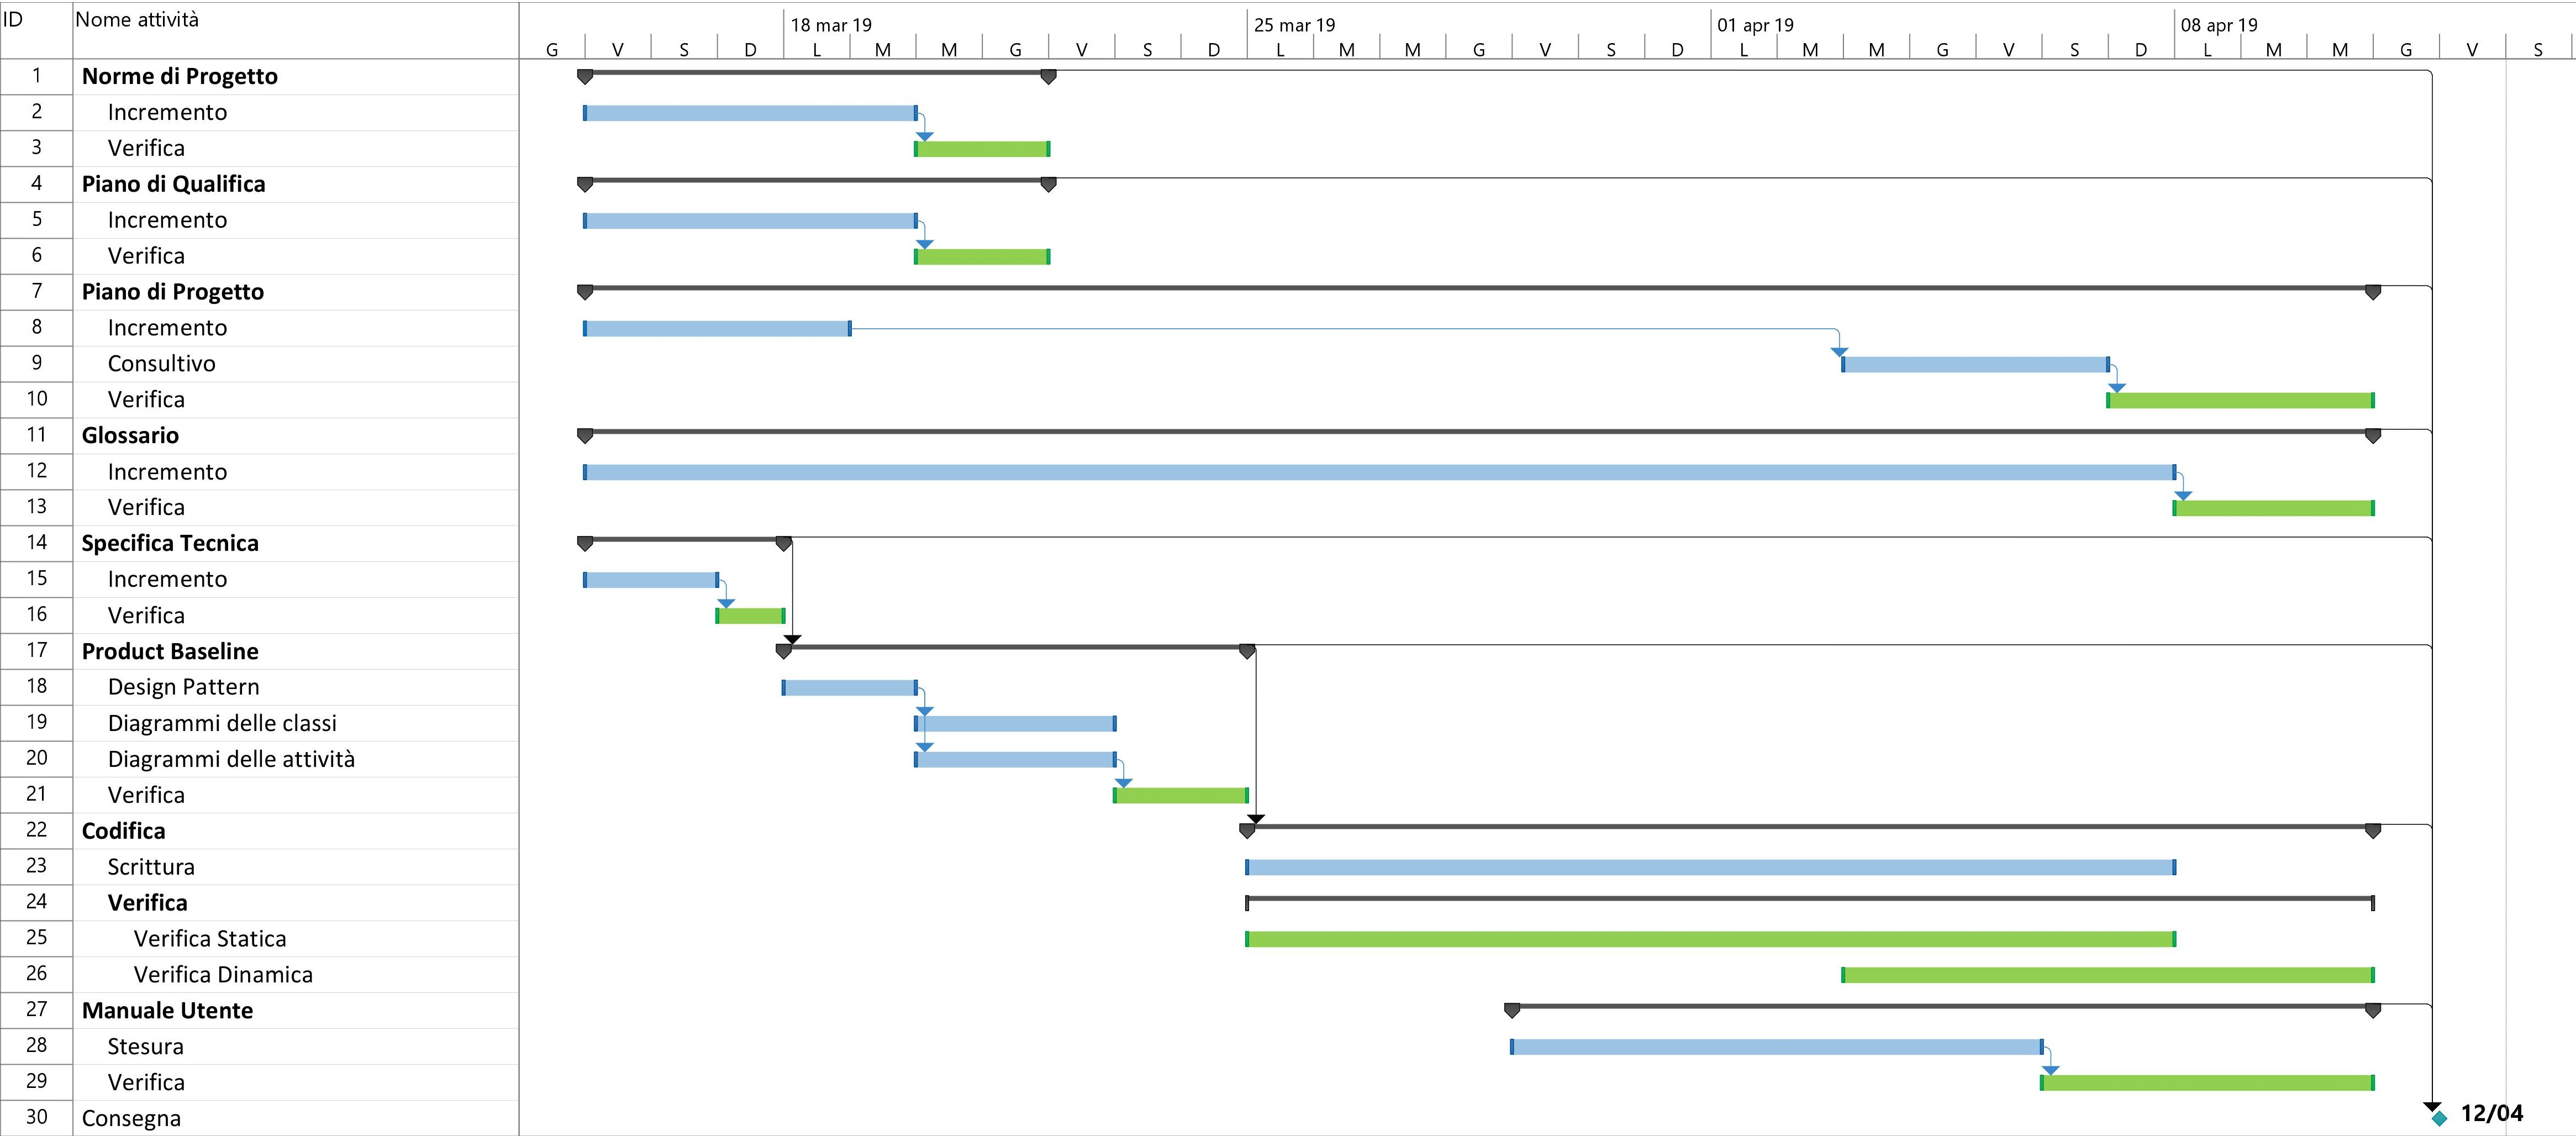
\includegraphics[width=0.99\linewidth]{res/images/gantt_pd.jpg}
	\caption{Diagramma di Gantt della fase di Progettazione di dettaglio e codifica}
\end{figure}
\pagebreak

\subsection{Validazione e collaudo}
\textit{Periodo: dal 2019-04-12 al 2019-05-17 } \\
L'inizio di questa fase coincide col la data di consegna dei documenti per la 
\textit{Revisione di Qualifica}, mentre la data di fine coincide con la 
consegna in vista della \textit{Revisione di Accettazione}. Durante questo periodo 
si eseguiranno ulteriori attività di validazione e verifica. Le attività 
previste sono: 
\begin{itemize}
	\item \textbf{Validazione e Collaudo}: per la parte di collaudo si 
	eseguiranno ulteriori test sul prodotto, in modo da garantirne la 
	correttezza e stabilità. Per la parte di validazione, verrà 
	valutata la coerenza del prodotto e dei requisiti specificati nel documento 
	\textit{Analisi dei Requisiti} nella sua ultima versione;
	\item \textbf{Manuale Sviluppatore}: viene redatto il documento \textit{Manuale Sviluppartore} atto a fornire tutte le informazioni necessarie al mantenimento, manutenzione e ampliamento del prodotto finale;
	\item \textbf{Incremento e Verifica}: se necessario vengono migliorati i 
	documenti prodotti nelle fasi precedenti.
\end{itemize}
\begin{figure}[H]
	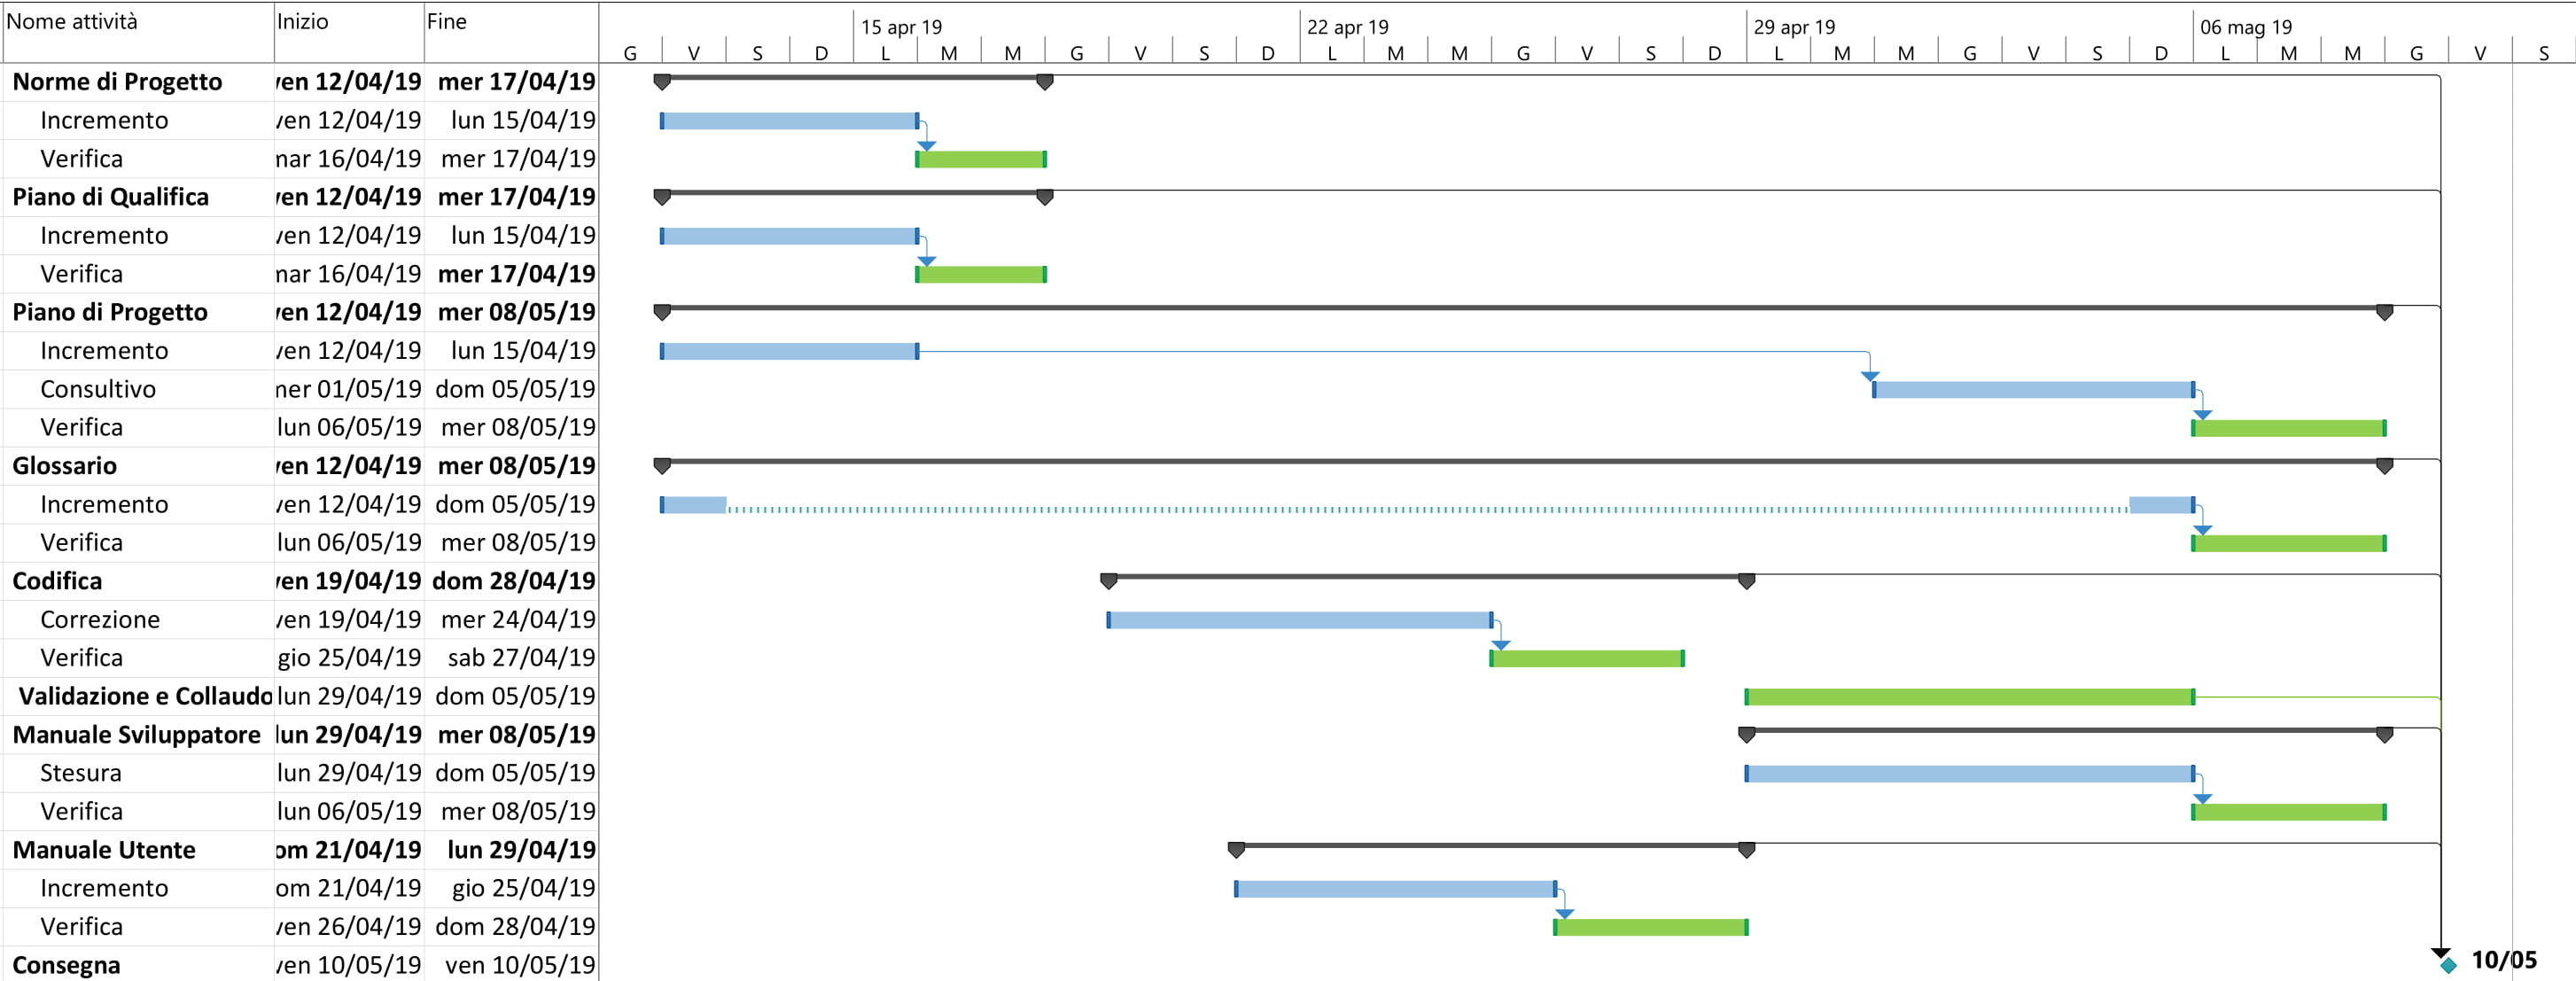
\includegraphics[width=0.99\linewidth]{res/images/gantt_val.jpg}
	\caption{Diagramma di Gantt della fase di validazione e collaudo}
\end{figure}

\pagebreak
% STA FACENDO SARA, NON TOCCARE
\section{Preventivo}
Per facilitare la lettura delle seguenti tabelle, vengono utilizzate delle sigle 
per identificare i ruoli:
\begin{itemize}
\item \textbf{Ad:} Amministratore;
\item \textbf{An:} Analista;
\item \textbf{Pj:} Progettista;
\item \textbf{Pr:} Programmatore;
\item \textbf{Re:} Responsabile;
\item \textbf{Ve:} Verificatore.
\end{itemize}
\noindent
Inoltre, se le ore ricoperte in un determinato ruolo fossero nulle, la cella 
presenterà il simbolo \textbf{-} per indicarne l'assenza. 

\subsection{Fase di Analisi}
\subsubsection{Prospetto orario}
In questa fase\glo{}, ogni componente del gruppo rivestirà i seguenti ruoli:
\begin{table}[H]
				\centering\renewcommand{\arraystretch}{1.5}
				\arrayrulecolor{white}
                \begin{tabular}{c|c|c|c|c|c|c|c}
                               
                \rowcolorhead
                 {\colorhead \textbf{Nominativo}} &
                 {\colorhead \textbf{Re}} & 
                 {\colorhead \textbf{Am}} & 
                 {\colorhead\textbf{An}} & 
                 {\colorhead \textbf{Pt}} & 
                 {\colorhead\textbf{Pr}} & 
                 {\colorhead \textbf{Ve}} & 
                 {\colorhead \textbf{Ore totali} }\\
				
                \rowcolorlight
                 {\colorbody Federico Bicciato} & {\colorbody 6} & 
                 {\colorbody 9} & {\colorbody -} & {\colorbody -} & 
                 {\colorbody -} & {\colorbody 4} & {\colorbody 19} 
				\\
				
				\rowcolordark
                 {\colorbody Mattia Bolzonella} & {\colorbody -} & 
                 {\colorbody -} & {\colorbody 12} & {\colorbody -} & 
                 {\colorbody -} & {\colorbody 7} & {\colorbody 19} 
				\\	
				
				\rowcolorlight
                 {\colorbody Francesco Donè} & {\colorbody 6} & 
                 {\colorbody -} & {\colorbody 8} & {\colorbody -} & 
                 {\colorbody -} & {\colorbody 5} & {\colorbody 19} 
				\\
				              
                \rowcolordark
                 {\colorbody Sara Feltrin} & {\colorbody -} & 
                 {\colorbody 5} & {\colorbody 10} & {\colorbody -} & 
                 {\colorbody -} & {\colorbody 4} & {\colorbody 19} 
				\\
				
				\rowcolorlight
                 {\colorbody Giacomo Greggio} & {\colorbody 6} & 
                 {\colorbody -} & {\colorbody 10} & {\colorbody -} & 
                 {\colorbody -} & {\colorbody 3} & {\colorbody 19} 
				\\
				
				\rowcolordark
                 {\colorbody Samuele Piazzetta} & {\colorbody -} & 
                 {\colorbody -} & {\colorbody 14} & {\colorbody -} & 
                 {\colorbody -} & {\colorbody 5} & {\colorbody 19} 
				\\	
				
				\rowcolorlight
                 {\colorbody Paolo Pozzan} & {\colorbody -} & 
                 {\colorbody 5} & {\colorbody 6} & {\colorbody -} & 
                 {\colorbody -} & {\colorbody 8} & {\colorbody 19} 
				\\
				
				\rowcolordark
                 {\colorbody Matteo Santinon} & {\colorbody 5} & 
                 {\colorbody -} & {\colorbody 8} & {\colorbody -} & 
                 {\colorbody -} & {\colorbody 5} & {\colorbody 18} 
				\\
				
				\rowcolorlight
                 {\colorbody \textbf{Ore totali ruolo}} & {\colorbody 23} & 
                 {\colorbody 19} & {\colorbody 68} & {\colorbody -} & 
                 {\colorbody -} & {\colorbody 41} & {\colorbody 151} 
				\\
                

                \end{tabular}
                \caption{Distribuzione delle ore nel periodo di Analisi}
\end{table}

I dati ottenuti si possono riassumere nel seguente istogramma:
\begin{figure}[H] 
			\centering 
				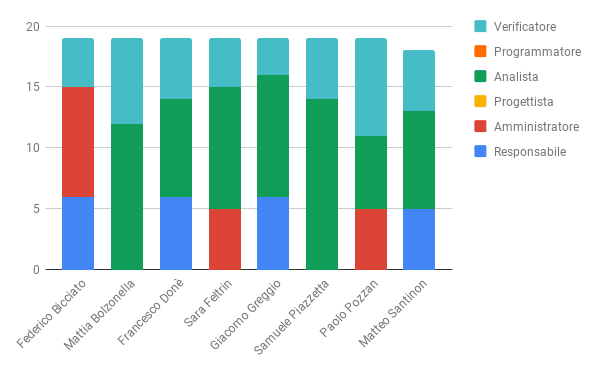
\includegraphics[width=0.7\textwidth]{res/images/istogramma_analisi.png}\\
				\caption{Istogramma della ripartizione di ore per ruolo in Analisi}
			\label{IstogrammaAnalisi}
\end{figure}


\subsubsection{Prospetto economico}
In questa fase il costo per ogni ruolo è il seguente:
\begin{table}[H]
				\centering\renewcommand{\arraystretch}{1.5}
				\arrayrulecolor{white}
                \begin{tabular}{c|c|c}
                               
                \rowcolorhead
                 {\colorhead \textbf{Ruolo}} &
                 {\colorhead \textbf{Ore}} & 
                 {\colorhead \textbf{Costo}} \\
				
                \rowcolorlight
                 {\colorbody Responsabile} & {\colorbody 23} & 
                 {\colorbody \EUR{690.00}}  
				\\
				
				\rowcolordark
                 {\colorbody Amministratore} & {\colorbody 19} & 
                 {\colorbody \EUR{380.00}}
				\\	
				
				\rowcolorlight
                 {\colorbody Analista} & {\colorbody 68} & 
                 {\colorbody \EUR{1,700.00}} 
				\\
				
				\rowcolordark
                 {\colorbody Progettista} & {\colorbody -} & 
                 {\colorbody -} 
				\\
				
				\rowcolorlight
                 {\colorbody Programmatore} & {\colorbody -} & 
                 {\colorbody -} 
				\\
				
				\rowcolordark
                 {\colorbody Verificatore} & {\colorbody 41} & 
                 {\colorbody \EUR{615.00}} 
				\\
				
				\rowcolorlight
                 {\colorbody \textbf{Totale}} & {\colorbody 151} & 
                 {\colorbody \EUR{3,385.00}} 
				\\
				
                

                \end{tabular}
                \caption{Prospetto dei costi per ruoli nel periodo di Analisi}
\end{table}

I dati ottenuti si possono riassumere nel seguente areogramma:
\begin{figure}[H] 
			\centering 
				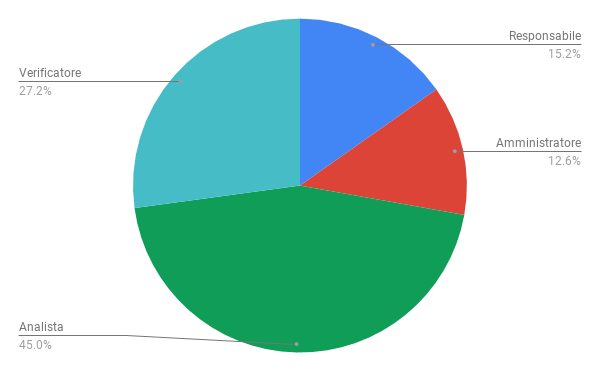
\includegraphics[width=0.5\textwidth]{res/images/areogramma_analisi.png}\\
				\caption{Areogramma della ripartizione di ore per ruolo in Analisi}
			\label{AreogrammaAnalisi}
\end{figure}

\subsection{Fase di Consolidamento dei requisiti}
\subsubsection{Prospetto orario}
Il periodo di Consolidamento dei requisiti vede la seguente distribuzione oraria:
\begin{table}[H]
				\centering\renewcommand{\arraystretch}{1.5}
				\arrayrulecolor{white}
                \begin{tabular}{c|c|c|c|c|c|c|c}
                               
                \rowcolorhead
                 {\colorhead \textbf{Nominativo}} &
                 {\colorhead \textbf{Re}} & 
                 {\colorhead \textbf{Am}} & 
                 {\colorhead\textbf{An}} & 
                 {\colorhead \textbf{Pt}} & 
                 {\colorhead\textbf{Pr}} & 
                 {\colorhead \textbf{Ve}} & 
                 {\colorhead \textbf{Ore totali} }\\
				
                \rowcolorlight
                 {\colorbody Federico Bicciato} & {\colorbody -} & 
                 {\colorbody -} & {\colorbody 5} & {\colorbody -} & 
                 {\colorbody -} & {\colorbody -} & {\colorbody 5} 
				\\
				
				\rowcolordark
                 {\colorbody Mattia Bolzonella} & {\colorbody -} & 
                 {\colorbody 5} & {\colorbody -} & {\colorbody -} & 
                 {\colorbody -} & {\colorbody -} & {\colorbody 5} 
				\\	
				
				\rowcolorlight
                 {\colorbody Francesco Donè} & {\colorbody -} & 
                 {\colorbody -} & {\colorbody 3} & {\colorbody -} & 
                 {\colorbody -} & {\colorbody 3} & {\colorbody 6} 
				\\
				
				\rowcolordark
                 {\colorbody Sara Feltrin} & {\colorbody 5} & 
                 {\colorbody -} & {\colorbody -} & {\colorbody -} & 
                 {\colorbody -} & {\colorbody -} & {\colorbody 5} 
				\\
                
                \rowcolorlight
                 {\colorbody Giacomo Greggio} & {\colorbody -} & 
                 {\colorbody -} & {\colorbody -} & {\colorbody -} & 
                 {\colorbody -} & {\colorbody 6} & {\colorbody 6} 
				\\
				
				\rowcolordark
                 {\colorbody Samuele Piazzetta} & {\colorbody -} & 
                 {\colorbody 3} & {\colorbody -} & {\colorbody -} & 
                 {\colorbody -} & {\colorbody 3} & {\colorbody 6} 
				\\	
				
				\rowcolorlight
                 {\colorbody Paolo Pozzan} & {\colorbody -} & 
                 {\colorbody -} & {\colorbody 4} & {\colorbody -} & 
                 {\colorbody -} & {\colorbody 2} & {\colorbody 6} 
				\\
				
				\rowcolordark
                 {\colorbody Matteo Santinon} & {\colorbody -} & 
                 {\colorbody -} & {\colorbody -} & {\colorbody -} & 
                 {\colorbody -} & {\colorbody 6} & {\colorbody 6} 
				\\
				
				\rowcolorlight
                 {\colorbody \textbf{Ore totali ruolo}} & {\colorbody 5} & 
                 {\colorbody 8} & {\colorbody 12} & {\colorbody -} & 
                 {\colorbody -} & {\colorbody 20} & { \colorbody 45} 
				\\

                \end{tabular}
                \caption{Distribuzione delle ore nel periodo di Consolidamento 
				dei requisiti}

\end{table}

I dati ottenuti si possono riassumere nel seguente istogramma:
\begin{figure}[H] 
			\centering 
				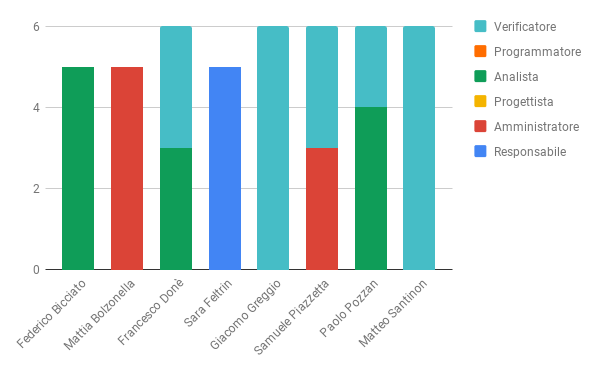
\includegraphics[width=0.7\textwidth]{res/images/istogramma_consolidamento.png}\\
				\caption{Istogramma della ripartizione di ore per ruolo in Consolidamento dei requisiti}
			\label{IstogrammaConsolidamento}
\end{figure}

\subsubsection{Prospetto economico}
In questa fase il costo per ogni ruolo è il seguente:
\begin{table}[H]
				\centering\renewcommand{\arraystretch}{1.5}
				\arrayrulecolor{white}
                \begin{tabular}{c|c|c}
                               
                \rowcolorhead
                 {\colorhead \textbf{Ruolo}} &
                 {\colorhead \textbf{Ore}} & 
                 {\colorhead \textbf{Costo}} \\
				
                \rowcolorlight
                 {\colorbody Responsabile} & {\colorbody 5} & 
                 {\colorbody \EUR{150.00}}  
				\\
				
				\rowcolordark
                 {\colorbody Amministratore} & {\colorbody 8} & 
                 {\colorbody \EUR{160.00}}
				\\	
				
				\rowcolorlight
                 {\colorbody Analista} & {\colorbody 12} & 
                 {\colorbody \EUR{300.00}} 
				\\
				
				\rowcolordark
                 {\colorbody Progettista} & {\colorbody -} & 
                 {\colorbody -} 
				\\
				
				\rowcolorlight
                 {\colorbody Programmatore} & {\colorbody -} & 
                 {\colorbody -} 
				\\
				
				\rowcolordark
                 {\colorbody Verificatore} & {\colorbody 20} & 
                 {\colorbody \EUR{300.00}} 
				\\
				
				\rowcolorlight
                 {\colorbody \textbf{Totale}} & {\colorbody 45} & 
                 {\colorbody \EUR{910.00}} 
				\\
                

                \end{tabular}
                \caption{Prospetto dei costi per ruoli nel periodo di 
				Consolidamento dei requisiti}

\end{table}

I dati ottenuti si possono riassumere nel seguente areogramma:
\begin{figure}[H] 
			\centering 
				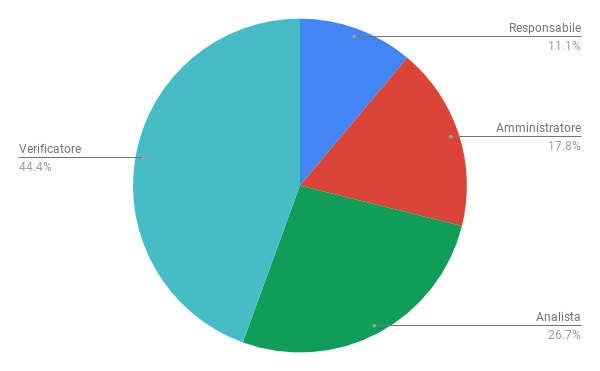
\includegraphics[width=0.5\textwidth]{res/images/areogramma_consolidamento.png}\\
				\caption{Areogramma della ripartizione di ore per ruolo in Consolidamento dei requisiti}
			\label{AreogrammaConsolidaemnto}
\end{figure}

\subsection{Fase di Progettazione architetturale}
\subsubsection{Prospetto orario}
Nella fase di Progettazione architetturale la distribuzione oraria è la seguente:
\begin{table}[H]
				\centering\renewcommand{\arraystretch}{1.5}
				\arrayrulecolor{white}
                \begin{tabular}{c|c|c|c|c|c|c|c}
                               
                \rowcolorhead
                 {\colorhead \textbf{Nominativo}} &
                 {\colorhead \textbf{Re}} & 
                 {\colorhead \textbf{Am}} & 
                 {\colorhead\textbf{An}} & 
                 {\colorhead \textbf{Pt}} & 
                 {\colorhead\textbf{Pr}} & 
                 {\colorhead \textbf{Ve}} & 
                 {\colorhead \textbf{Ore totali} }\\
				
                \rowcolorlight
                 {\colorbody Federico Bicciato} & {\colorbody -} & 
                 {\colorbody -} & {\colorbody 12} & {\colorbody -} & 
                 {\colorbody -} & {\colorbody 12} & {\colorbody 24} 
				\\
				
				\rowcolordark
                 {\colorbody Mattia Bolzonella} & {\colorbody 6} & 
                 {\colorbody -} & {\colorbody -} & {\colorbody 8} & 
                 {\colorbody -} & {\colorbody 10} & {\colorbody 24} 
				\\	
				
				\rowcolorlight
                 {\colorbody Francesco Donè} & {\colorbody -} & 
                 {\colorbody -} & {\colorbody -} & {\colorbody 12} & 
                 {\colorbody -} & {\colorbody 12} & {\colorbody 24} 
				\\
				
				\rowcolordark
                 {\colorbody Sara Feltrin} & {\colorbody -} & 
                 {\colorbody -} & {\colorbody -} & {\colorbody 14} & 
                 {\colorbody -} & {\colorbody 10} & {\colorbody 24} 
				\\
                
                \rowcolorlight
                 {\colorbody Giacomo Greggio} & {\colorbody -} & 
                 {\colorbody -} & {\colorbody -} & {\colorbody 13} & 
                 {\colorbody -} & {\colorbody 10} & {\colorbody 23} 
				\\
				
				\rowcolordark
                 {\colorbody Samuele Piazzetta} & {\colorbody 2} & 
                 {\colorbody 3} & {\colorbody -} & {\colorbody 18} & 
                 {\colorbody -} & {\colorbody -} & {\colorbody 24} 
				\\	
				
				\rowcolorlight
                 {\colorbody Paolo Pozzan} & {\colorbody -} & 
                 {\colorbody -} & {\colorbody -} & {\colorbody 18} & 
                 {\colorbody -} & {\colorbody 6} & {\colorbody 24} 
				\\
				
				\rowcolordark
                 {\colorbody Matteo Santinon} & {\colorbody -} & 
                 {\colorbody 7} & {\colorbody 6} & {\colorbody 11} & 
                 {\colorbody -} & {\colorbody -} & {\colorbody 24} 
				\\
				
				\rowcolorlight
                 {\colorbody \textbf{Ore totali ruolo}} & {\colorbody 8} & 
                 {\colorbody 10} & {\colorbody 18} & {\colorbody 94} & 
                 {\colorbody -} & {\colorbody 60} & {\colorbody 190} 
				\\

                \end{tabular}
                \caption{Distribuzione delle ore nel periodo di Progettazione 
				architetturale}

\end{table}

Una rappresentazione visiva della suddivisione oraria viene data dal seguente grafico:
\begin{figure}[H] 
			\centering 
				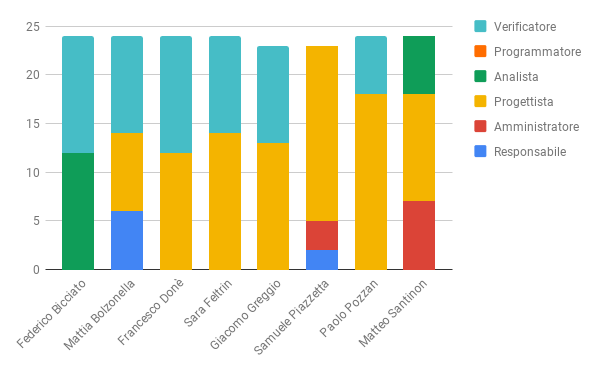
\includegraphics[width=0.7\textwidth]{res/images/istogramma_architetturale.png}\\
				\caption{Istogramma della ripartizione di ore per ruolo in Progettazione architetturale}
			\label{IstogrammaArchitetturale}
\end{figure}

\subsubsection{Prospetto economico}
In questa fase il costo per ogni ruolo è il seguente:
\begin{table}[H]
				\centering\renewcommand{\arraystretch}{1.5}
				\arrayrulecolor{white}
                \begin{tabular}{c|c|c}
                               
                \rowcolorhead
                 {\colorhead \textbf{Ruolo}} &
                 {\colorhead \textbf{Ore}} & 
                 {\colorhead \textbf{Costo}} \\
				
                \rowcolorlight
                 {\colorbody Responsabile} & {\colorbody 8} & 
                 {\colorbody \EUR{240.00}}  
				\\
				
				\rowcolordark
                 {\colorbody Amministratore} & {\colorbody 10} & 
                 {\colorbody \EUR{200.00}}
				\\	
				
				\rowcolorlight
                 {\colorbody Analista} & {\colorbody 18} & 
                 {\colorbody \EUR{450.00}} 
				\\
				
				\rowcolordark
                 {\colorbody Progettista} & {\colorbody 94} & 
                 {\colorbody \EUR{2,068.00}} 
				\\
				
				\rowcolorlight
                 {\colorbody Programmatore} & {\colorbody -} & 
                 {\colorbody -} 
				\\
				
				\rowcolordark
                 {\colorbody Verificatore} & {\colorbody 60} & 
                 {\colorbody \EUR{900.00}} 
				\\
				
				\rowcolorlight
                 {\colorbody \textbf{Totale}} & {\colorbody 190} & 
                 {\colorbody \EUR{3,858.00}} 
				\\
                

                \end{tabular}
                \caption{Prospetto dei costi per ruoli nel periodo di 
				Progettazione architetturale}

\end{table}
I dati ottenuti si possono riassumere nel seguente areogramma:
\begin{figure}[H] 
			\centering 
				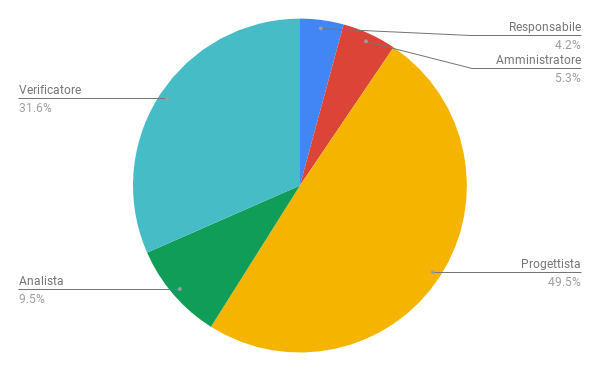
\includegraphics[width=0.5\textwidth]{res/images/areogramma_architetturale.png}\\
				\caption{Areogramma della ripartizione di ore per ruolo in Progettazione architetturale}
			\label{AreogrammaArchitetturale}
\end{figure}

\subsection{Fase di Progettazione di dettaglio e codifica}
\subsubsection{Prospetto orario}
Nella fase di Progettazione di dettaglio e codifica la distribuzione oraria è la seguente:
\begin{table}[H]
				\centering\renewcommand{\arraystretch}{1.5}
				\arrayrulecolor{white}
                \begin{tabular}{c|c|c|c|c|c|c|c}
                               
                \rowcolorhead
                 {\colorhead \textbf{Nominativo}} &
                 {\colorhead \textbf{Re}} & 
                 {\colorhead \textbf{Am}} & 
                 {\colorhead\textbf{An}} & 
                 {\colorhead \textbf{Pt}} & 
                 {\colorhead\textbf{Pr}} & 
                 {\colorhead \textbf{Ve}} & 
                 {\colorhead \textbf{Ore totali} }\\
				
                \rowcolorlight
                 {\colorbody Federico Bicciato} & {\colorbody -} & 
                 {\colorbody -} & {\colorbody -} & {\colorbody 16} & 
                 {\colorbody 17} & {\colorbody 9} & {\colorbody 42} 
				\\
				
				\rowcolordark
                 {\colorbody Mattia Bolzonella} & {\colorbody -} & 
                 {\colorbody -} & {\colorbody -} & {\colorbody 11} & 
                 {\colorbody 18} & {\colorbody 13} & {\colorbody 42} 
				\\	
				
				\rowcolorlight
                 {\colorbody Francesco Donè} & {\colorbody -} & 
                 {\colorbody -} & {\colorbody -} & {\colorbody 15} & 
                 {\colorbody 17} & {\colorbody 9} & {\colorbody 41} 
				\\
				
				\rowcolordark
                 {\colorbody Sara Feltrin} & {\colorbody -} & 
                 {\colorbody -} & {\colorbody 4} & {\colorbody 12} & 
                 {\colorbody 17} & {\colorbody 9} & { \colorbody 42} 
				\\
                
                \rowcolorlight
                 {\colorbody Giacomo Greggio} & {\colorbody -} & 
                 {\colorbody 8} & {\colorbody -} & {\colorbody 12} & 
                 {\colorbody 10} & {\colorbody 12} & {\colorbody 42} 
				\\
				
				\rowcolordark
                 {\colorbody Samuele Piazzetta} & {\colorbody 6} & 
                 {\colorbody -} & {\colorbody -} & {\colorbody 13} & 
                 {\colorbody 8} & {\colorbody 15} & {\colorbody 42} 
				\\	
				
				\rowcolorlight
                 {\colorbody Paolo Pozzan} & {\colorbody 8} & 
                 {\colorbody -} & {\colorbody -} & {\colorbody 11} & 
                 {\colorbody 18} & {\colorbody 4} & {\colorbody 41} 
				\\
				
				\rowcolordark
                 {\colorbody Matteo Santinon} & {\colorbody -} & 
                 {\colorbody -} & {\colorbody -} & {\colorbody 18} & 
                 {\colorbody 16} & {\colorbody 8} & {\colorbody 42} 
				\\
				
				\rowcolorlight
                 {\colorbody \textbf{Ore totali ruolo}} & {\colorbody 14} & 
                 {\colorbody 8} & {\colorbody 4} & {\colorbody 108} & 
                 {\colorbody 121} & {\colorbody 79} & {\colorbody 334} 
				\\

                \end{tabular}
                \caption{Distribuzione delle ore nel periodo di Progettazione di 
				dettaglio e codifica}

\end{table}

Una rappresentazione visiva della suddivisione oraria viene data dal seguente grafico:
\begin{figure}[H] 
			\centering 
				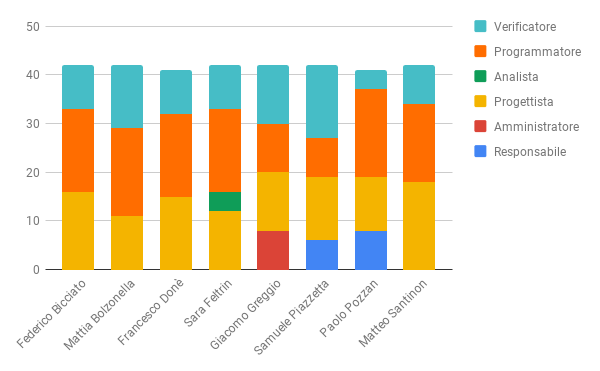
\includegraphics[width=0.5\textwidth]{res/images/istogramma_dettaglio.png}\\
				\caption{Istogramma della ripartizione di ore per ruolo in Progettazione di dettaglio e codifica}
			\label{IstogrammaDettaglio}
\end{figure}

\subsubsection{Prospetto economico}
In questa fase il costo per ogni ruolo è il seguente:
\begin{table}[H]
				\centering\renewcommand{\arraystretch}{1.5}
				\arrayrulecolor{white}
                \begin{tabular}{c|c|c}
                               
                \rowcolorhead
                 {\colorhead \textbf{Ruolo}} &
                 {\colorhead \textbf{Ore}} & 
                 {\colorhead \textbf{Costo}} \\
				
                \rowcolorlight
                 {\colorbody Responsabile} & {\colorbody 14} & 
                 {\colorbody \EUR{420.00}}  
				\\
				
				\rowcolordark
                 {\colorbody Amministratore} & {\colorbody 8} & 
                 {\colorbody \EUR{160.00}}
				\\	
				
				\rowcolorlight
                 {\colorbody Analista} & {\colorbody 4} & 
                 {\colorbody \EUR{100.00}} 
				\\
				
				\rowcolordark
                 {\colorbody Progettista} & {\colorbody 108} & 
                 {\colorbody \EUR{2,376.00}} 
				\\
				
				\rowcolorlight
                 {\colorbody Programmatore} & {\colorbody 121} & 
                 {\colorbody \EUR{1,815.00}} 
				\\
				
				\rowcolordark
                 {\colorbody Verificatore} & {\colorbody 79} & 
                 {\colorbody \EUR{1,185.00}} 
				\\
				
				\rowcolorlight
                 {\colorbody \textbf{Totale}} & {\colorbody 334} & 
                 {\colorbody \EUR{6,056.00}} 
				\\
                

                \end{tabular}
                \caption{Prospetto dei costi per ruoli nel periodo di 
				Progettazione di dettaglio e codifica}

\end{table}

I dati ottenuti si possono riassumere nel seguente areogramma:
\begin{figure}[H] 
			\centering 
				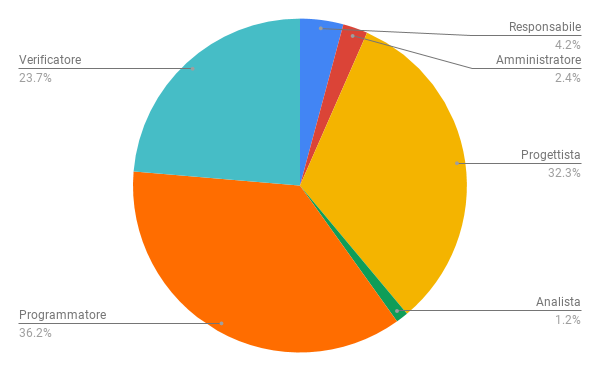
\includegraphics[width=0.5\textwidth]{res/images/areogramma_dettaglio.png}\\
				\caption{Areogramma della ripartizione di ore per ruolo in Progettazione di dettaglio e codifica}
			\label{AreogrammaDettaglio}
\end{figure}


\subsection{Fase di Validazione e collaudo}
\subsubsection{Prospetto orario}
Nella fase di progettazione di Validazione e collaudo la distribuzione oraria è la seguente:
\begin{table}[H]
				\centering\renewcommand{\arraystretch}{1.5}
				\arrayrulecolor{white}
                \begin{tabular}{c|c|c|c|c|c|c|c}
                               
                \rowcolorhead
                 {\colorhead \textbf{Nominativo}} &
                 {\colorhead \textbf{Re}} & 
                 {\colorhead \textbf{Am}} & 
                 {\colorhead\textbf{An}} & 
                 {\colorhead \textbf{Pt}} & 
                 {\colorhead\textbf{Pr}} & 
                 {\colorhead \textbf{Ve}} & 
                 {\colorhead \textbf{Ore totali} }\\
				
                \rowcolorlight
                 {\colorbody Federico Bicciato} & {\colorbody -} & 
                 {\colorbody -} & {\colorbody -} & {\colorbody 9} & 
                 {\colorbody -} & {\colorbody 6} & {\colorbody 15} 
				\\
				
				\rowcolordark
                 {\colorbody Mattia Bolzonella} & {\colorbody -} & 
                 {\colorbody 4} & {\colorbody -} & {\colorbody 11} & 
                 {\colorbody -} & {\colorbody -} & {\colorbody 15} 
				\\	
				
				\rowcolorlight
                 {\colorbody Francesco Donè} & {\colorbody 3} & 
                 {\colorbody 5} & {\colorbody -} & {\colorbody -} & 
                 {\colorbody 7} & {\colorbody -} & {\colorbody 15} 
				\\
				
				\rowcolordark
                 {\colorbody Sara Feltrin} & {\colorbody 4} & 
                 {\colorbody -} & {\colorbody -} & {\colorbody -} & 
                 {\colorbody -} & {\colorbody 11} & {\colorbody 15} 
				\\
                
                \rowcolorlight
                 {\colorbody Giacomo Greggio} & {\colorbody -} & 
                 {\colorbody -} & {\colorbody -} & {\colorbody -} & 
                 {\colorbody 7} & {\colorbody 8} & {\colorbody 15} 
				\\
				
				\rowcolordark
                 {\colorbody Samuele Piazzetta} & {\colorbody -} & 
                 {\colorbody -} & {\colorbody -} & {\colorbody -} & 
                 {\colorbody 9} & {\colorbody 6} & {\colorbody 15} 
				\\	
				
				\rowcolorlight
                 {\colorbody Paolo Pozzan} & {\colorbody -} & 
                 {\colorbody 3} & {\colorbody -} & {\colorbody -} & 
                 {\colorbody -} & {\colorbody 12} & {\colorbody 15} 
				\\
				
				\rowcolordark
                 {\colorbody Matteo Santinon} & {\colorbody 3} & 
                 {\colorbody -} & {\colorbody -} & {\colorbody -} & 
                 {\colorbody -} & {\colorbody 12} & {\colorbody 15} 
				\\
				
				\rowcolorlight
                 {\colorbody \textbf{Ore totali ruolo}} & {\colorbody 10} & 
                 {\colorbody 12} & {\colorbody 20} & {\colorbody -} & 
                 {\colorbody 23} & {\colorbody 55} & {\colorbody 120} 
				\\

                \end{tabular}
                \caption{Distribuzione delle ore nel periodo di Validazione e 
				collaudo}
\end{table}

Una rappresentazione visiva della suddivisione oraria viene data dal seguente grafico:
\begin{figure}[H] 
			\centering 
				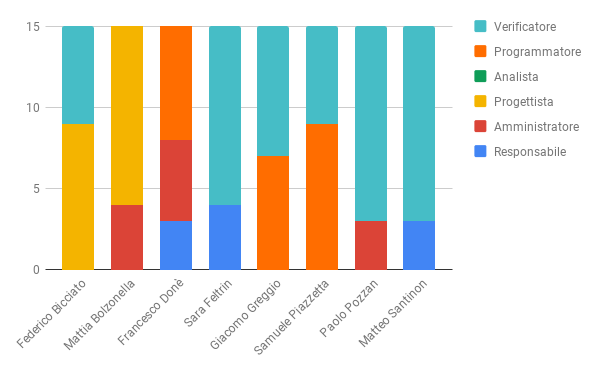
\includegraphics[width=0.5\textwidth]{res/images/istogramma_validazione.png}\\
				\caption{Istogramma della ripartizione di ore per ruolo in Validazione e collaudo}
			\label{IstogrammaValidazione}
\end{figure}

\subsubsection{Prospetto economico}
In questa fase il costo per ogni ruolo è il seguente:
\begin{table}[H]
				\centering\renewcommand{\arraystretch}{1.5}
				\arrayrulecolor{white}
                \begin{tabular}{c|c|c}
                               
                \rowcolorhead
                 {\colorhead \textbf{Ruolo}} &
                 {\colorhead \textbf{Ore}} & 
                 {\colorhead \textbf{Costo}} \\
				
                \rowcolorlight
                 {\colorbody Responsabile} & {\colorbody 10} & 
                 {\colorbody \EUR{300.00}}  
				\\
				
				\rowcolordark
                 {\colorbody Amministratore} & {\colorbody 12} & 
                 {\colorbody \EUR{240.00}}
				\\	
				
				\rowcolorlight
                 {\colorbody Analista} & {\colorbody 20} & 
                 {\colorbody \EUR{440.00}} 
				\\
				
				\rowcolordark
                 {\colorbody Progettista} & {\colorbody -} & 
                 {\colorbody -} 
				\\
				
				\rowcolorlight
                 {\colorbody Programmatore} & {\colorbody 23} & 
                 {\colorbody \EUR{345.00}} 
				\\
				
				\rowcolordark
                 {\colorbody Verificatore} & {\colorbody 55} & 
                 {\colorbody \EUR{825.00}} 
				\\
				
				\rowcolorlight
                 {\colorbody \textbf{Totale}} & {\colorbody 120} & 
                 {\colorbody \EUR{2,150.00}} 
				\\
                

                \end{tabular}
                \caption{Prospetto dei costi per ruoli nel periodo di 
				Validazione e collaudo}

\end{table}

I dati ottenuti si possono riassumere nel seguente areogramma:
\begin{figure}[H] 
			\centering 
				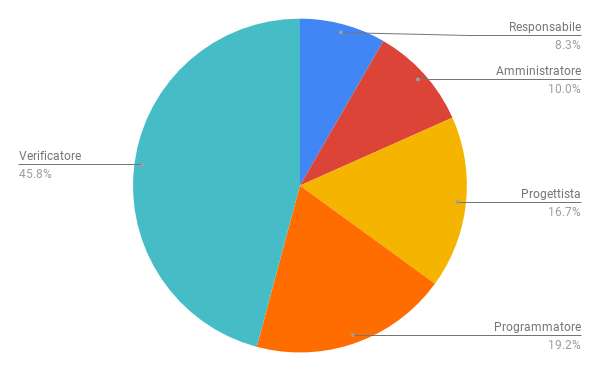
\includegraphics[width=0.5\textwidth]{res/images/areogramma_validazione.png}\\
				\caption{Areogramma della ripartizione di ore per ruolo in Validazione e collaudo}
			\label{AreogrammaValidazione}
\end{figure}


\subsection{Riepilogo}
\subsubsection{Ore totali}
\paragraph{Suddivisione del lavoro}\mbox{}\\
Vengono riportate il totale delle ore del progetto in cui sono presenti le ore di investimento e le ore rendicontate a carico del committente:
\begin{table}[H]
				\centering\renewcommand{\arraystretch}{1.5}
				\arrayrulecolor{white}
                \begin{tabular}{c|c|c|c|c|c|c|c}
                               
                \rowcolorhead
                 {\colorhead \textbf{Nominativo}} &
                 {\colorhead \textbf{Re}} & 
                 {\colorhead \textbf{Am}} & 
                 {\colorhead\textbf{An}} & 
                 {\colorhead \textbf{Pt}} & 
                 {\colorhead\textbf{Pr}} & 
                 {\colorhead \textbf{Ve}} & 
                 {\colorhead \textbf{Ore totali} }\\
				
                \rowcolorlight
                 {\colorbody Federico Bicciato} & {\colorbody 6} & 
                 {\colorbody 9} & {\colorbody 17} & {\colorbody 25} & 
                 {\colorbody 17} & {\colorbody 31} & {\colorbody 105} 
				\\
				
				\rowcolordark
                 {\colorbody Mattia Bolzonella} & {\colorbody 6} & 
                 {\colorbody 9} & {\colorbody 12} & {\colorbody 30} & 
                 {\colorbody 18} & {\colorbody 30} & {\colorbody 105} 
				\\	
				
				\rowcolorlight
                 {\colorbody Francesco Donè} & {\colorbody 9} & 
                 {\colorbody 5} & {\colorbody 11} & {\colorbody 27} & 
                 {\colorbody 24} & {\colorbody 29} & {\colorbody 105} 
				\\
				
				\rowcolordark
                 {\colorbody Sara Feltrin} & {\colorbody 9} & 
                 {\colorbody 5} & {\colorbody 15} & {\colorbody 26} & 
                 {\colorbody 17} & {\colorbody 34} & {\colorbody 105} 
				\\
                
                \rowcolorlight
                 {\colorbody Giacomo Greggio} & {\colorbody 6} & 
                 {\colorbody 8} & {\colorbody 10} & {\colorbody 25} & 
                 {\colorbody 17} & {\colorbody 39} & {\colorbody 105} 
				\\
				
				\rowcolordark
                 {\colorbody Samuele Piazzetta} & {\colorbody 8} & 
                 {\colorbody 6} & {\colorbody 14} & {\colorbody 31} & 
                 {\colorbody 17} & {\colorbody 29} & {\colorbody 105} 
				\\	
				
				\rowcolorlight
                 {\colorbody Paolo Pozzan} & {\colorbody 8} & 
                 {\colorbody 8} & {\colorbody 10} & {\colorbody 29} & 
                 {\colorbody 18} & {\colorbody 32} & {\colorbody 105} 
				\\
				
				\rowcolordark
                 {\colorbody Matteo Santinon} & {\colorbody 8} & 
                 {\colorbody 7} & {\colorbody 14} & {\colorbody 29} & 
                 {\colorbody 16} & {\colorbody 31} & {\colorbody 105} 
				\\
				
				\rowcolorlight
                 {\colorbody \textbf{Ore totali ruolo}} & {\colorbody 60} & 
                 {\colorbody 57} & {\colorbody 102} & {\colorbody 222} & 
                 {\colorbody144 } & {\colorbody 255} & {\colorbody 840} 
				\\

                \end{tabular}
                \caption{Distribuzione delle ore totali di investimento e rendicontate}

\end{table}

Una rappresentazione visiva della suddivisione oraria viene data dal seguente grafico:
\begin{figure}[H] 
			\centering 
				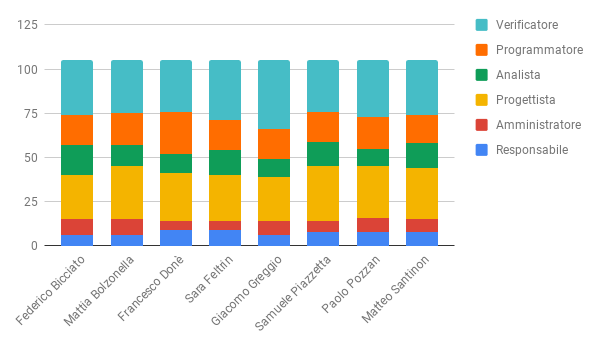
\includegraphics[width=0.5\textwidth]{res/images/istogramma_riepilogo.png}\\
				\caption{Istogramma della ripartizione di ore totali di investimento e rendicontate}
			\label{IstogrammaRiepilogo}
\end{figure}

\paragraph{Prospetto economico}\mbox{}\\
In questa fase il costo per ogni ruolo è il seguente:
\begin{table}[H]
				\centering\renewcommand{\arraystretch}{1.5}
				\arrayrulecolor{white}
                \begin{tabular}{c|c|c}
                               
                \rowcolorhead
                 {\colorhead \textbf{Ruolo}} &
                 {\colorhead \textbf{Ore}} & 
                 {\colorhead \textbf{Costo}} \\
				
                \rowcolorlight
                 {\colorbody Responsabile} & {\colorbody 60} & 
                 {\colorbody \EUR{1,800.00}}  
				\\
				
				\rowcolordark
                 {\colorbody Amministratore} & {\colorbody 57} & 
                 {\colorbody \EUR{1,140.00}}
				\\	
				
				\rowcolorlight
                 {\colorbody Analista} & {\colorbody 102} & 
                 {\colorbody \EUR{2,550.00}} 
				\\
				
				\rowcolordark
                 {\colorbody Progettista} & {\colorbody 222} & 
                 {\colorbody \EUR{4,884.00}} 
				\\
				
				\rowcolorlight
                 {\colorbody Programmatore} & {\colorbody 144} & 
                 {\colorbody \EUR{2,160.00}} 
				\\
				
				\rowcolordark
                 {\colorbody Verificatore} & {\colorbody 255} & 
                 {\colorbody \EUR{3,825.00}} 
				\\
				
				\rowcolorlight
                 {\colorbody \textbf{Totale}} & {\colorbody 840} & 
                 {\colorbody \EUR{16,359.00}} 
				\\
                

                \end{tabular}
                \caption{Prospetto dei costi totale delle ore di investimento e rendicontate}

\end{table}

I dati ottenuti si possono riassumere nel seguente diagramma:
\begin{figure}[H] 
			\centering 
				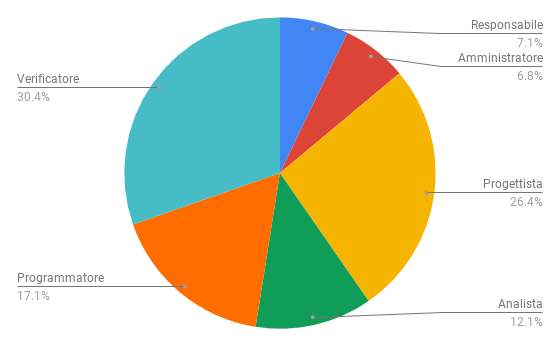
\includegraphics[width=0.5\textwidth]{res/images/areogramma_riepilogo.png}\\
				\caption{Areogramma dei costi totale delle ore di investimento e rendicontate}
			\label{AreogrammaRiepilogoRuoli}
\end{figure}


\subsubsection{Ore rendicontate}
\paragraph{Suddivisione del lavoro}\mbox{}\\
\linebreak
Le ore rendicontate sono riassunte nella seguente tabella:
\begin{table}[H]
				\centering\renewcommand{\arraystretch}{1.5}
				\arrayrulecolor{white}
                \begin{tabular}{c|c|c|c|c|c|c|c}
                               
                \rowcolorhead
                 {\colorhead \textbf{Nominativo}} &
                 {\colorhead \textbf{Re}} & 
                 {\colorhead \textbf{Am}} & 
                 {\colorhead\textbf{An}} & 
                 {\colorhead \textbf{Pt}} & 
                 {\colorhead\textbf{Pr}} & 
                 {\colorhead \textbf{Ve}} & 
                 {\colorhead \textbf{Ore totali} }\\
				
                \rowcolorlight
                 {\colorbody Federico Bicciato} & {\colorbody 6} & 
                 {\colorbody 4} & {\colorbody 12} & {\colorbody 22} & 
                 {\colorbody 17} & {\colorbody 30} & {\colorbody 91} 
				\\
				
				\rowcolordark
                 {\colorbody Mattia Bolzonella} & {\colorbody 4} & 
                 {\colorbody 6} & {\colorbody 10} & {\colorbody 30} & 
                 {\colorbody 18} & {\colorbody 23} & {\colorbody 91} 
				\\	
				
				\rowcolorlight
                 {\colorbody Francesco Donè} & {\colorbody 9} & 
                 {\colorbody 5} & {\colorbody 10} & {\colorbody 23} & 
                 {\colorbody 23} & {\colorbody 21} & {\colorbody 91} 
				\\
				
				\rowcolordark
                 {\colorbody Sara Feltrin} & {\colorbody 5} & 
                 {\colorbody 5} & {\colorbody 14} & {\colorbody 26} & 
                 {\colorbody 14} & {\colorbody 27} & {\colorbody 91} 
				\\
                
                \rowcolorlight
                 {\colorbody Giacomo Greggio} & {\colorbody 4} & 
                 {\colorbody 8} & {\colorbody 10} & {\colorbody 23} & 
                 {\colorbody 12} & {\colorbody 34} & {\colorbody 91} 
				\\
				
				\rowcolordark
                 {\colorbody Samuele Piazzetta} & {\colorbody 6} & 
                 {\colorbody 6} & {\colorbody 12} & {\colorbody 28} & 
                 {\colorbody 13} & {\colorbody 26} & {\colorbody 91} 
				\\	
				
				\rowcolorlight
                 {\colorbody Paolo Pozzan} & {\colorbody 8} & 
                 {\colorbody 5} & {\colorbody 10} & {\colorbody 25} & 
                 {\colorbody 16} & {\colorbody 27} & {\colorbody 91} 
				\\
				
				\rowcolordark
                 {\colorbody Matteo Santinon} & {\colorbody 5} & 
                 {\colorbody 7} & {\colorbody 14} & {\colorbody 27} & 
                 {\colorbody 14} & {\colorbody 24} & {\colorbody 91} 
				\\
				
				\rowcolorlight
                 {\colorbody \textbf{Ore totali ruolo}} & {\colorbody 47} & 
                 {\colorbody 49} & {\colorbody 92} & {\colorbody 204} & 
                 {\colorbody 127} & {\colorbody 212} & {\colorbody 728} 
				\\

                \end{tabular}
                \caption{Distribuzione delle ore rendicontate}

\end{table}

\begin{figure}[H] 
			\centering 
				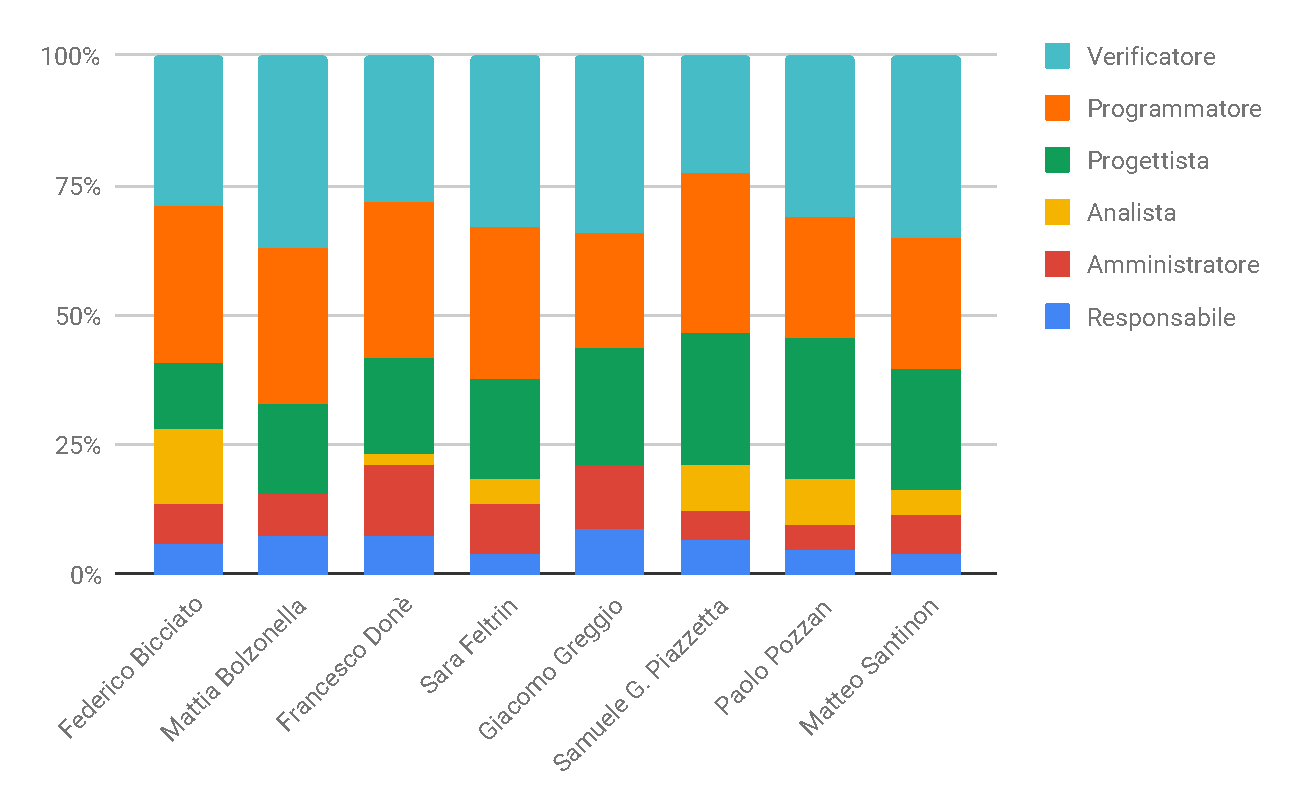
\includegraphics[width=0.5\textwidth]{res/images/istogramma_rendicontate.pdf}\\
				\caption{Istogramma della ripartizione delle ore rendicontate}
			\label{IstogrammaOreRendicontate}
\end{figure}

\paragraph{Prospetto economico}\mbox{}\\
\linebreak
Il totale rendicontato dei costi sostenuti per ogni ruolo è riassunto nella seguente tabella:

\begin{table}[H]
				\centering\renewcommand{\arraystretch}{1.5}
				\arrayrulecolor{white}
                \begin{tabular}{c|c|c}
                               
                \rowcolorhead
                 {\colorhead \textbf{Ruolo}} &
                 {\colorhead \textbf{Ore}} & 
                 {\colorhead \textbf{Costo}} \\
				
                \rowcolorlight
                 {\colorbody Responsabile} & {\colorbody 47} & 
                 {\colorbody \EUR{1,410.00}}  
				\\
				
				\rowcolordark
                 {\colorbody Amministratore} & {\colorbody 46} & 
                 {\colorbody \EUR{920.00}}
				\\	
				
				\rowcolorlight
                 {\colorbody Analista} & {\colorbody 92} & 
                 {\colorbody \EUR{2,300.00}} 
				\\
				
				\rowcolordark
                 {\colorbody Progettista} & {\colorbody 204} & 
                 {\colorbody \EUR{4,488.00}} 
				\\
				
				\rowcolorlight
                 {\colorbody Programmatore} & {\colorbody 127} & 
                 {\colorbody \EUR{1,905.00}} 
				\\
				
				\rowcolordark
                 {\colorbody Verificatore} & {\colorbody 212} & 
                 {\colorbody \EUR{3,180.00}} 
				\\
				
				\rowcolorlight
                 {\colorbody \textbf{Totale}} & {\colorbody 728} & 
                 {\colorbody \EUR{14,203.00}} 
				\\
                

                \end{tabular}
                \caption{Prospetto dei costi delle ore rendicontate}

\end{table}

I dati ottenuti si possono riassumere nel seguente diagramma:
\begin{figure}[H] 
			\centering 
				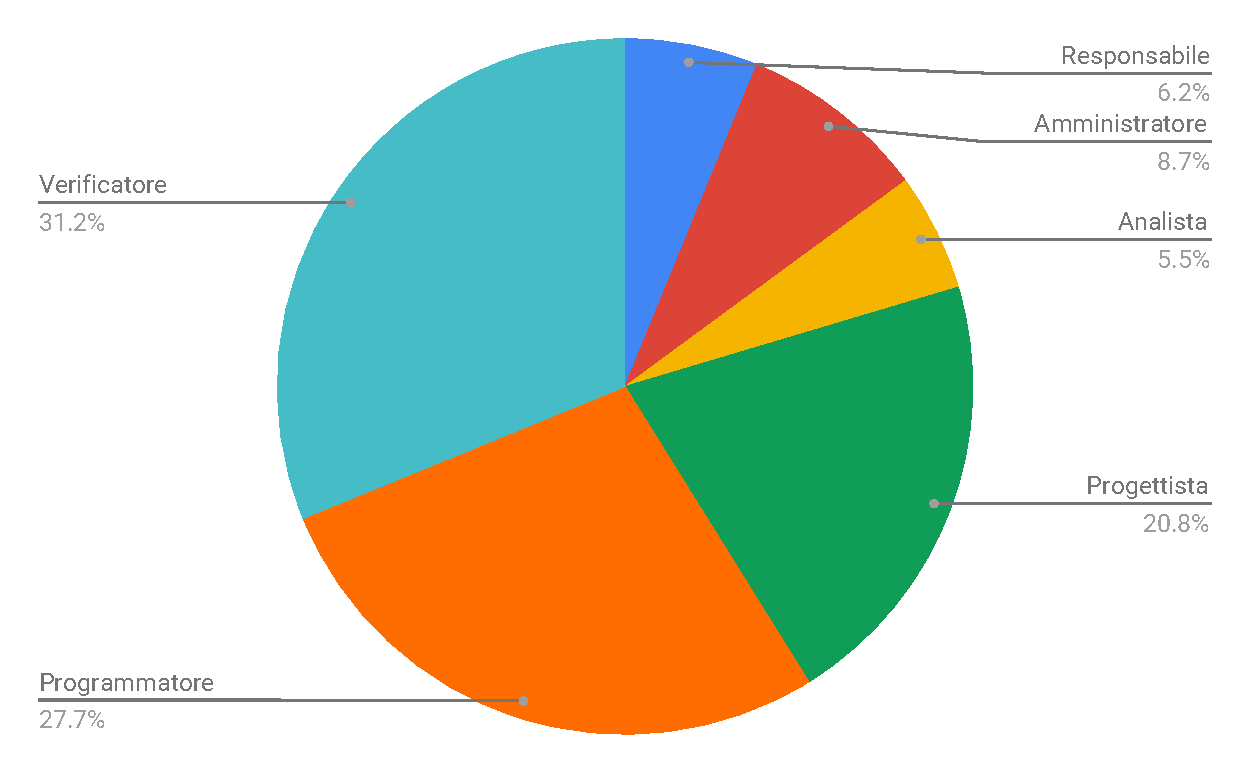
\includegraphics[width=0.5\textwidth]{res/images/areogramma_rendicontate.pdf}\\
				\caption{Areogramma delle ore rendicontate per ruolo}
			\label{AreogrammaOreRendicontate}
\end{figure}

\subsubsection{Conclusioni}
Il costo totale preventivato per il progetto è \EUR{14,203.00}.



\pagebreak
\section{Consuntivi di periodo}
Di seguito verranno indicate le spese effettivamente sostenute, considerando sia quelle per ruolo sia quelle per persona. Il bilancio potrà risultare:
\begin{itemize}
	\item \textbf{Negativo:} se il consuntivo supera il preventivo;
	\item \textbf{Pari:} se il consuntivo e il preventivo sono pari;
	\item \textbf{Positivo:} se il preventivo supera il consuntivo.
\end{itemize}

\subsection{Periodo di analisi}
Le ore di lavoro sostenute in questa fase sono da considerarsi come ore di investimento per l'approfondimento personale. Esse sono quindi non rendicontate.

\begin{table}[H]
				\centering\renewcommand{\arraystretch}{1.5}
				\caption{Consuntivo di periodo della fase di Analisi}
				\vspace{0.2cm}
                \begin{tabular}{c c c}
                               
                \rowcolorhead
                 {\colorhead \textbf{Ruolo}} &
                 {\colorhead \textbf{Ore}} & 
                 {\colorhead \textbf{Costo}} \\
				
                \rowcolorlight
                 {\colorbody Responsabile} & {\colorbody 31 (+0)} & 
                 {\colorbody \EUR{930,00} (+\EUR{0,00})}  
				\\
				
				\rowcolordark
                 {\colorbody Amministratore} & {\colorbody 44 (+19)} & 
                 {\colorbody \EUR{880,00} (+\EUR{380,00})}
				\\	
				
				\rowcolorlight
                 {\colorbody Analista} & {\colorbody 96 (+7)} & 
                 {\colorbody \EUR{2.400,00} (+\EUR{175,00})} 
				\\
				
				\rowcolordark
                 {\colorbody Progettista} & {\colorbody 19
                 (+7)} & 
                 {\colorbody \EUR{418,00} (+\EUR{154,00})} 
				\\
				
				\rowcolorlight
                 {\colorbody Programmatore} & {\colorbody -} & 
                 {\colorbody -} 
				\\
				
				\rowcolordark
                 {\colorbody Verificatore} & {\colorbody 90 (+7)} & 
                 {\colorbody \EUR{1.350,00} (+\EUR{105,00})} 
				\\
				
				\rowcolorlight
                 {\colorbody \textbf{Totale Preventivo}} & {\colorbody \textbf{280}} & 
                 {\colorbody \textbf{\EUR{5.978,00}}} 
				\\
				
				
				\rowcolordark
                 {\colorbody \textbf{Totale Consuntivo}} & {\colorbody \textbf{320}} & 
                 {\colorbody \textbf{\EUR{6.792,00}}} 
				\\
				
				
				\rowcolorlight
                 {\colorbody \textbf{Differenza}} & {\colorbody \textbf{40}} & 
                 {\colorbody \textbf{\EUR{+814,00}}} 
				\\
				
                

                \end{tabular}
                
\end{table}

\subsubsection{Conclusioni}
Come emerge dai dati riportati nella tabella soprastante, che presenta le ore relative al consuntivo della fase di Analisi, è stato necessario investire più tempo del previsto nei ruoli di \textit{Amministratore}, \textit{Analista}, \textit{Progettista} e \textit{Verificatore}. Per questo motivo il bilancio risultante è negativo. Di seguito sono riportate le cause di tali ritardi:
\begin{itemize}
	\item \textbf{\textit{Amministratori}}: è servito più tempo del previsto per riuscire ad individuare i software più adatti per la gestione del progetto, e per la loro corretta configurazione. Inoltre sono state aggiunte ed aggiornate alcune sezioni nelle \textit{Norme di Progetto}, necessarie al chiarimento di alcune problematiche sorte durante la stesura dei documenti;
	\item \textbf{\textit{Analisti}}: alcuni requisiti si sono rivelati di non facile comprensione, e sono state necessarie più ore di lavoro per la discussione interna (tra gli \textit{Analisti)} ed esterna (con i proponenti); 
	\item \textbf{\textit{Progettisti}}: l'elevato numero di requisiti individuati nell'\textit{Analisi dei Requisiti} ha comportato un aumento del tempo necessario alla stesura dei test;
	\item \textbf{\textit{Verificatori}}: l'aggiunta di nuove sezioni nelle Norme di Progetto e l'elevato numero di requisiti individuati hanno implicato un maggiore lavoro anche per questo ruolo. 
\end{itemize}
Il notevole quantitativo di ore che il gruppo ha dovuto impiegare nel primo periodo non deve ripetersi durante il lavoro rendicontato. Per le problematiche riscontrate verranno adottate le seguenti contromisure:
\begin{itemize}
	\item \textbf{configurazione della strumentazione}: buona parte degli strumenti sono già stati configurati. La configurazione della rimanente strumentazione verrà effettuata all'inizio della seconda fase, al fine di evitare un successivo consumo di ore per uniformare la strumentazione stessa ed i prodotti dei diversi elementi del gruppo;
	\item \textbf{comprensione dei requisiti}: i requisiti sono stati ampiamente discussi con il proponente durante questa fase, non si prevede di incorrere ulteriormente in tale problema;
	\item \textbf{scorretta implementazione ed utilizzo iniziale delle Norme di Progetto}: il gruppo ha finito la stesura del documento ed ha imparato ad applicare le norme in esso definite.
\end{itemize}

\subsubsection{Preventivo a finire} 
Essendo il primo periodo non rendicontato, non è necessario prevedere alcuna contromisura dal punto di vista del monte ore totale nonché del preventivo economico. I componenti del gruppo dovranno adottare le contromisure sopra descritte e lavorare con il metodo acquisito durante questo primo periodo.

\subsection{Periodo di consolidamento dei requisiti}
Le ore di lavoro sostenute in questa periodo sono relative al consolidamento dei requisiti, successivo al periodo di analisi. Alcune ore sono state dedicate allo studio per l'approfondimento personale e sono da considerarsi come ore non rendicontate. Per tale motivo tali ore non sono state riportate nella seguente tabella.

\begin{table}[H]
	\centering\renewcommand{\arraystretch}{1.5}
	\caption{Consuntivo di periodo della fase di Consolidamento dei requisiti}
	\vspace{0.2cm}
	\begin{tabular}{c c c}
		
		\rowcolorhead
		{\colorhead \textbf{Ruolo}} &
		{\colorhead \textbf{Ore}} & 
		{\colorhead \textbf{Costo}} \\
		
		\rowcolorlight
		{\colorbody Responsabile} & {\colorbody 3 (+0)} & 
		{\colorbody \EUR{90,00} (+\EUR{0,00})}  
		\\
		
		\rowcolordark
		{\colorbody Amministratore} & {\colorbody 5 (+0)} & 
		{\colorbody \EUR{100,00} (+\EUR{0,00})}
		\\	
		
		\rowcolorlight
		{\colorbody Analista} & {\colorbody 15 (+0)} & 
		{\colorbody \EUR{375,00} (+\EUR{0,00})} 
		\\
		
		\rowcolordark
		{\colorbody Progettista} & {\colorbody -
			} & 
		{\colorbody -} 
		\\
		
		\rowcolorlight
		{\colorbody Programmatore} & {\colorbody -} & 
		{\colorbody -} 
		\\
		
		\rowcolordark
		{\colorbody Verificatore} & {\colorbody 17 (+0)} & 
		{\colorbody \EUR{255,00} (+\EUR{0,00})} 
		\\
		
		\rowcolorlight
		{\colorbody \textbf{Totale Preventivo}} & {\colorbody \textbf{40}} & 
		{\colorbody \textbf{\EUR{820,00}}} 
		\\
		
		
		\rowcolordark
		{\colorbody \textbf{Totale Consuntivo}} & {\colorbody \textbf{40}} & 
		{\colorbody \textbf{\EUR{820,00}}} 
		\\
		
		
		\rowcolorlight
		{\colorbody \textbf{Differenza}} & {\colorbody \textbf{-}} & 
		{\colorbody \textbf{-}} 
		\\
		
		
		
	\end{tabular}
	
\end{table}

\subsubsection{Conclusioni}
Come emerge dai dati riportati nelle tabella soprastante, le ore di lavoro effettivamente impiegate dai diversi ruoli coincidono con quanto riportato nel preventivo. Il gruppo, diversamente dal periodo di Analisi dei requisiti, è riuscito a rientrare nelle ore di lavoro preventivate. Tale miglioramento nella gestione della mole di lavoro è causato, oltre alla ridotta durata di tale periodo, all'esperienza guadagnata dai membri nel primo periodo.

\subsubsection{Preventivo a finire} 
Considerando che le ore effettivamente utilizzate coincidono con quelle preventivate, ed essendo il periodo in considerazione non rendicontato, non è necessario prendere alcun accorgimento e/o modificare i preventivi riguardanti i periodi rimanenti.

\subsection{Periodo di progettazione e codifica per la Technology Baseline}
Le ore sostenute durante questo periodo sono relative alla progettazione ed alla codifica del Proof of Concept\glo, necessario al soddisfacimento della Techology Baseline\glo. Tale periodo, successivo al Consolidamento dei requisiti, è da considerarsi rendicontato, in quanto il capitolato d'appalto è stato aggiudicato e quindi il lavoro è svolto con lo scopo di sviluppare il prodotto finale. 

\begin{table}[H]
	\centering\renewcommand{\arraystretch}{1.5}
	\caption{Consuntivo di periodo della fase di Progettazione e Codifica per la Technology Baseline}
	\vspace{0.2cm}
	\begin{tabular}{c c c}
		
		\rowcolorhead
		{\colorhead \textbf{Ruolo}} &
		{\colorhead \textbf{Ore}} & 
		{\colorhead \textbf{Costo}} \\
		
		\rowcolorlight
		{\colorbody Responsabile} & {\colorbody 10 (+2)} & 
		{\colorbody \EUR{300,00} (+\EUR{60,00})}  
		\\
		
		\rowcolordark
		{\colorbody Amministratore} & {\colorbody 22 (+10)} & 
		{\colorbody \EUR{440,00} (+\EUR{200,00})}
		\\	
		
		\rowcolorlight
		{\colorbody Analista} & {\colorbody 30 (+0)} & 
		{\colorbody \EUR{750,00} (+\EUR{0,00})} 
		\\
		
		\rowcolordark
		{\colorbody Progettista} & {\colorbody 67
			(-32)} & 
		{\colorbody \EUR{1474,00} (-\EUR{704,00})} 
		\\
		
		\rowcolorlight
		{\colorbody Programmatore} & {\colorbody 30 (+50)} & 
		{\colorbody \EUR{450,00} (+\EUR{750,00})} 
		\\
		
		\rowcolordark
		{\colorbody Verificatore} & {\colorbody 65 (-30)} & 
		{\colorbody \EUR{975,00} (-\EUR{450,00})} 
		\\
		
		\rowcolorlight
		{\colorbody \textbf{Totale Preventivo}} & {\colorbody \textbf{224}} & 
		{\colorbody \textbf{\EUR{4.389,00}}} 
		\\
		
		
		\rowcolordark
		{\colorbody \textbf{Totale Consuntivo}} & {\colorbody \textbf{224}} & 
		{\colorbody \textbf{\EUR{4.245,00}}} 
		\\
		
		
		\rowcolorlight
		{\colorbody \textbf{Differenza}} & {\colorbody \textbf{0}} & 
		{\colorbody \textbf{\EUR{-144,00}}} 
		\\
		
		
		
	\end{tabular}
	
\end{table}

\subsubsection{Conclusioni}
Dai dati riportati nella tabella soprastante si evince che la progettazione riguardante tale periodo ha subito una sostanziale modifica. Il gruppo aveva infatti pianificato di redarre una completa progettazione architetturale del prodotto, e di riportarla all'interno di un documento formale. Tuttavia il lavoro svolto durante questo periodo si è concentrato maggiormente sul verificare, attraverso la progettazione e la codifica del Proof of Concept\glo, che le tecnologie scelte si integrassero efficacemente tra loro, e che grazie al loro utilizzo i requisiti potessero essere soddisfatti. Di seguito sono riportate le motivazioni delle variazioni del monte ore di lavoro ricoperto dai diversi ruoli:

\begin{itemize}
	\item \textbf{\textit{Amministratori}}: dopo aver testato l'editor precedentemente stabilito, sono stati riscontrati alcuni problemi riguardanti dei plug-in\glosp necessari allo sviluppo del software. La conseguente decisione di cambiare l'editor ha comportato la necessità di ore aggiuntive di lavoro da parte degli amministratori. Un'altra causa di tale scostamento dalle ore preventivate sono alcune difficoltà riscontrate nel set-up del sistema di Continuous Integration\glo;
	\item \textbf{\textit{Progettisti}}: visto il cambiamento dell'obiettivo finale di tale periodo, i progettisti hanno dovuto occuparsi solamente di alcune componenti del prodotto finale. Ciò ha richiesto molto meno tempo rispetto a quanto preventivato;
	\item \textbf{\textit{Programmatori}}: visto il cambiamento dell'obiettivo finale di tale periodo, la quantità di ore assegnate al ruolo di programmatore ha subito un notevole aumento. Parte dell'ammontare è stato aggiunto per risolvere alcune problematiche nate dall'utilizzo delle ultime versioni di alcuni framework\glosp utilizzati. Questi infatti contenevano dei bug non risolti e/o scarsa documentazione;
	\item \textbf{\textit{Verificatori}}: il cambiamento dell'obiettivo di tale periodo ha comportato una diminuzione delle ore dedicate alla verifica. Era stata preventivata infatti la redazione di un documento aggiuntivo, che non è stato più redatto.
\end{itemize}
Le ore di lavoro relative ai ruoli che hanno subito delle variazioni rispetto a quanto pianificato sono state distribuite in maniera tale che ogni elemento del gruppo svolgesse lo stesso monte ore di lavoro complessivo.
\subsubsection{Preventivo a finire} 
Il bilancio economico risultante è positivo, ovvero sono stati risparmiati {\EUR{144,00}. Tali fondi verranno impiegati nei prossimi periodi per far fronte ad eventuali ritardi o per implementare i requisiti opzionali.
	
\subsection{Periodo di progettazione di dettaglio e codifica}
Le ore sostenute durante questo periodo sono relative alla redazione alla codifica necessaria 
per la realizzazione della Product Baseline\glo. Tale periodo è da considerarsi 
rendicontato in quanto il lavoro è svolto con lo scopo di sviluppare il prodotto finale.

\begin{table}[H]
	\centering\renewcommand{\arraystretch}{1.5}
	\caption{Consuntivo di periodo della fase di progettazione di dettaglio e codifica}
	\vspace{0.2cm}
	\begin{tabular}{c c c}
		\rowcolorhead
		{\colorhead \textbf{Ruolo}} &
		{\colorhead \textbf{Ore}} & 
		{\colorhead \textbf{Costo}} \\
		
		\rowcolorlight
		{\colorbody Responsabile} & {\colorbody 21(+0)} & 
		{\colorbody \EUR{630,00} (+\EUR{0,00})}  
		\\
		
		\rowcolordark
		{\colorbody Amministratore} & {\colorbody 29(+0)} & 
		{\colorbody \EUR{580,00} (+\EUR{0,00})}
		\\	
		
		\rowcolorlight
		{\colorbody Analista} & {\colorbody 0(+4)} & 
		{\colorbody \EUR{0,00} (+\EUR{100,00})} 
		\\
		
		\rowcolordark
		{\colorbody Progettista} & {\colorbody 90(+30)} & 
		{\colorbody \EUR{1980,00} (+\EUR{660,00})} 
		\\
		
		\rowcolorlight
		{\colorbody Programmatore} & {\colorbody 157(-27)} & 
		{\colorbody \EUR{2355,00} (-\EUR{405,00})} 
		\\
		
		\rowcolordark
		{\colorbody Verificatore} & {\colorbody 103(+0)} & 
		{\colorbody \EUR{1545,00} (+\EUR{0,00})} 
		\\
		
		\rowcolorlight
		{\colorbody \textbf{Totale Preventivo}} & {\colorbody \textbf{400}} & 
		{\colorbody \textbf{\EUR{7.090,00}}} 
		\\
		
		\rowcolordark
		{\colorbody \textbf{Totale Consuntivo}} & {\colorbody \textbf{407}} & 
		{\colorbody \textbf{\EUR{7.445,00}}} 
		\\
		
		\rowcolorlight
		{\colorbody \textbf{Differenza}} & {\colorbody \textbf{7}} & 
		{\colorbody \textbf{\EUR{+355,00}}} 
		\\
		
		\rowcolordark
		{\colorbody \textbf{Totale con risparmio(-\EUR{144,00})}} &  & 
		{\colorbody \textbf{\EUR{211,00}}} 
		\\	
	\end{tabular}
\end{table}

\subsubsection{Conclusioni}
Dai dati riportati nella tabella soprastante si evince che la progettazione ha subito una sostanziale modifica, di conseguenza le ore del programmatore hanno subito un notevole ridimensionamento. 
Di seguito sono riportate le problematiche sorte durante questa fase di lavoro e le motivazioni degli scostamenti del mantenimento del monte ore di 
lavoro preventivato:
\begin{itemize}
	\item \textbf{\textit{Amministratori}}: alcuni problemi si sono riscontrati durante il settaggio di Solidity-coverage, fortunatamente risolti in tempi contenuti senza comportare un aumento delle ore;
	\item \textbf{\textit{Analisti}}: sono state aggiunte alcune ore all'Analista non preventivate, in quanto c'è stato bisogno di effettuare le correzioni segnalate sull'\textit{Analisi dei Requisiti} e, come indicato nel \textit{Piano di Qualifica v3.0.0}, alcune ore sono state dedicate al supporto dei Progettisti nella stesura di diagrammi relativi alla progettazione;
	\item \textbf{\textit{Progettisti}}: alcuni problemi si sono riscontrati con l'identificazione dei design pattern da applicare al backend, in quanto per incompatibilità, si è dovuto procedere con la ricerca di ulteriori pattern, oltre a quelli studiati a lezione. Inoltre si sono riscontrate difficoltà nella progettazione dei moduli per l'ottimizzazione delle transazioni e nella sicurezza legata all'accesso ai dati. Nella definizione dei prodotti si sono riscontrati problemi legati a limiti del linguaggio Solidity, dunque si è deciso di utilizzare nuovi costrutti e di portare delle modifica della logica. L'introduzione di IPFS ha richiesto un numero di ore necessario allo studio della tecnologia;
	\item \textbf{\textit{Programmatori}}: a seguito di quanto specificato relativamente alla progettazione, la programmazione ha subito un periodo di stallo in attesa del termine della rivisitazione della progettazione e la risoluzione dei problemi con Solidity. D'altra parte, una volta terminata la rivisitazione della progettazione, è stato possibile procedere più rapidamente nel lavoro di implementazione.
\end{itemize}
\subsubsection{Preventivo a finire}
Il bilancio economico risultante è negativo, mitigato dal fatto di aver un fondo cuscinetto dalla fase precedente di \EUR{144,00} che porta ad avere una perdita di \EUR{211,00}. Tale perdita sarà tenuta in considerazione nella fase successiva, in quanto si prevede di recuperare il debito grazie alla rivisitazione della progettazione effettuata che ci consentirà di risparmiare ore nella fase di testing e codifica in generale che attualmente si trova ad uno stato avanzato.
\\


\pagebreak
\appendix
\section{Organigramma}

\subsection{Redazione}
\begin{table}[H]
	\centering\renewcommand{\arraystretch}{1.5}
	\arrayrulecolor{white}
    \begin{tabular}{c|c|c}
		\hline
		
		\rowcolorhead 
		{\colorhead \textbf{Nominativo}} &
		{\colorhead \textbf{Data di redazione}} &
		{\colorhead \textbf{Firma}}  \\ 
		
		\rowcolorlight
		Sara Feltrin & 2019-01-08 &   \\ 
		\rowcolordark
		Mattia Bolzonella & 2019-01-08 &   \\ 
		\rowcolorlight
		Matteo Santinon & 2019-01-08 &   \\ 
	\end{tabular}
	\caption{Redazione}
\end{table}

\subsection{Approvazione}
\begin{table}[H]
	\centering\renewcommand{\arraystretch}{1.5}
	\arrayrulecolor{white}
	\begin{tabular}{c|c|c}
		\hline
		
		\rowcolorhead 
		{\colorhead \textbf{Nominativo}} &
		{\colorhead \textbf{Data di approvazione}} &
		{\colorhead \textbf{Firma}}  \\
		
		\rowcolorlight
		Giacomo Greggio & 2019-01-10 &   \\ 
		\rowcolordark
		Tullio Vardanega &  &   \\ 
		\rowcolorlight
		Riccardo Cardin &  &   \\ 
	\end{tabular}
	\caption{Approvazione}
\end{table}

\subsection{Accettazione dei componenti}
\begin{table}[H]
	\centering\renewcommand{\arraystretch}{1.5}
	\arrayrulecolor{white}
	\begin{tabular}{c|c|c}
		\hline
		
		\rowcolorhead 
		{\colorhead \textbf{Nominativo}} &
		{\colorhead \textbf{Data di accettazione}} &
		{\colorhead \textbf{Firma}}  \\
		
		\rowcolorlight
		Federico Bicciato & 2018-11-16 &   \\ \hline
		\rowcolordark
		Mattia Bolzonella & 2018-11-16 &   \\ \hline
		\rowcolorlight
		Francesco Donè & 2018-11-16 &   \\ \hline
		\rowcolordark
		Sara Feltrin & 2018-11-16 &   \\ \hline
		\rowcolorlight
		Giacomo Greggio & 2018-11-16 &   \\ \hline
		\rowcolordark
		Samuele Piazzetta & 2018-11-16 &   \\ \hline
		\rowcolorlight
		Paolo Pozzan & 2018-11-16 &   \\ \hline
		\rowcolordark
		Matteo Santinon & 2018-11-16 &   \\ \hline
	\end{tabular}
	\caption{Accettazione dei componenti}
\end{table}

\subsection{Componenti}
\begin{table}[H]
	\centering\renewcommand{\arraystretch}{1.5}
	\arrayrulecolor{white}
	\begin{tabular}{c|c|c}
		\hline
		
		\rowcolorhead 
		{\colorhead \textbf{Nominativo}} &
		{\colorhead \textbf{Matricola}} &
		{\colorhead \textbf{Indirizzo di posta elettronica}}  \\
		
		\rowcolorlight
		Federico Bicciato & 1046373 & federico.bicciato.1@studenti.unipd.it  \\ \hline
		\rowcolordark
		Mattia Bolzonella & 1123066 & mattia.bolzonella@studenti.unipd.it  \\ \hline
		\rowcolorlight
		Francesco Donè & 1142196 & francesco.done@studenti.unipd.it  \\ \hline
		\rowcolordark
		Sara Feltrin & 1122453 &  sara.feltrin.2@studenti.unipd.it \\ \hline
		\rowcolorlight
		Giacomo Greggio &  &   \\ \hline
		\rowcolordark
		Samuele Giuliano Piazzetta & 1144219  & samuelegiuliano.piazzetta@studenti.unipd.it  \\ \hline
		\rowcolorlight
		Paolo Pozzan & 1121339  &  paolo.pozzan@studenti.unipd.it  \\ \hline
		\rowcolordark
		Matteo Santinon & 1122298 &  matteo.santinon.1@studenti.unipd.it \\ \hline
	\end{tabular}
	\caption{Accettazione dei componenti}
\end{table}


\pagebreak
\section{Attualizzazione dei rischi}

\rowcolors{2}{pari}{dispari}
\renewcommand{\arraystretch}{1.5}
\begin{longtable}{
		 >{\centering}p{0.17\textwidth}
		 >{\centering}p{0.37\textwidth}
		 >{\centering}p{0.37\textwidth}
	 }
 	\caption{Tabella dei }\\
 	
	\rowcolorhead 
		\textbf{\color{white}Rischio}	& \textbf{\color{white}Descrizione} &
		\textbf{\color{white}Contromisura adottata}
		\tabularnewline 		
	\endhead
	Inesperienza tecnologica RT1 & 
	I programmatori hanno riscontrato alcuni bug nell'ultima release di un framework\glosp utilizzato. & 
	È stato deciso di utilizzare una versione precedente di tale framework\glosp che non presentava i bug individuati.
	\tabularnewline
	
	Impegni Accademici RO3 &
	Tutti i componenti del gruppo hanno dovuto sostenere alcuni esami. Pertanto, in alcuni periodi non tutti i componenti hanno potuto dare la propria disponibilità. &
	Le task più onerose sono state assegnate alle persone momentaneamente più disponibili.
	
	
	
\end{longtable}


\end{document}
